%%%%%%%%%%%%%%%%%%%%%%%%%%%%%%%%%%%%%%%%%%%%%%%%%%%%%%%%%%%%%%%%%%%%%%%%%%%%%%%%%%%%%%%%%%%%%%%%%%%%%%%%%%%%%%%%%%%%%%%%%%%%%%%%%%%%%%%
%%Latexvorlage by Pascal Enderli, Zürich
%%%%%%%%%%%%%%%%%%%%%%%%%%%%%%%%%%%%%%%%%%%%%%%%%%%%%%%%%%%%%%%%%%%%%%%%%%%%%%%%%%%%%%%%%%%%%%%%%%%%%%%%%%%%%%%%%%%%%%%%%%%%%%%%%%%%%%%
%% Diese Vorlage enthät alle nötigen tools um ein grosses Projekt (Bachelorarbeit, Masterarbeit) zu verfassen.
%% Unter anderem ist enthalten:
%% -struktur einer wissenschaftlichen arbeit
%% -abbildungs-,tabellen-,literatur-,akronym- und symbolverzeichnis
%% -Makefile für offlinekompilierung (Linuxuser) ausführen mit ./make.sh im obersten ordner
%% -einige befehle und hinweise für die verwendung von referenzen aller art im file:
%% ./mainmatter/introduction.tex und ./backmatter/literature.bib
%%%%%%%%%%%%%%%%%%%%%%%%%%%%%%%%%%%%%%%%%%%%%%%%%%%%%%%%%%%%%%%%%%%%%%%%%%%%%%%%%%%%%%%%%%%%%%%%%%%%%%%%%%%%%%%%%%%%%%%%%%%%%%%%%%%%%%%
%% Bemerkungen:
%% Das Skript darf natürlich nach euren wünschen angepasst und wiederveröffentlicht werden
%% Bei der Erstellung des Literaturverzeichnisses habe ich biber verwendet (weil utf-8 kompatibel),
%% welches vor dem kompilieren nachinstalliert werden muss falls noch nicht vorhanden (unter linux: sudo apt-get install biber )
%% alternativ kann man das projekt auf sharelatex.com hochladen und bearbeiten
%% (bitte sicher stellen dass das file ./frontmatter/glossaries.glo korrekt in sharelatex importiert wurde)
%% Dieses Skript verwendet KOMA-Skript 
%%%%%%%%%%%%%%%%%%%%%%%%%%%%%%%%%%%%%%%%%%%%%%%%%%%%%%%%%%%%%%%%%%%%%%%%%%%%%%%%%%%%%%%%%%%%%%%%%%%%%%%%%%%%%%%%%%%%%%%%%%%%%%%%%%%%%%%

\documentclass[
parskip=full,               %ganze leere linie vor neuen absatz <false(einzug),half halbe linie abstand>
headings=small,             %kleinere schrift bei den kopfzeilen
headsepline=0.3pt,          %separierungslinie für kopfzeile <dicke:länge>
footsepline=false,          %separierungslinie für fusszeile <dicke:länge>
plainheadsepline=true,      %separierungslinie für kopfzeile auch bei seite mit neuem kapitel
plainfootsepline=false,     %separierungslinie für fusszeile auch bei seite mit neuem kapitel
11pt,                       %schriftgrösse <10pt, 11pt, 12pt>
oneside,                    %modus einseitige seiten <twoside>
a4paper                     %a4 format
]{scrbook}                  %komaskript klasse scrbook


\usepackage{header}

%%%%%%%%%%%%%%%%%%%%%%%%%%%%%%%%%%%%%%%%%%%%%%%%%%%%%%%%%%%%%%%%%%%%%%%%%%%%%%%%%%%%%%%%%%%%%%%%
%auswählen welche files kompiliert werden sollen (Auskommentieren)

\includeonly{
 ./frontmatter/titlepage,
 ./frontmatter/abstract,
 ./frontmatter/note_of_thanks,
 % main 
 ./mainmatter/theory/studies_surveys,
 ./mainmatter/theory/comparable_works,
 ./mainmatter/theory/description_of_used_methods,
 ./mainmatter/theory/literary_studies,
 ./mainmatter/theory/description_of_env_and_domain,
 % development
./mainmatter/development/power_of_the_dot,
./mainmatter/development/iterables_everywhere,
./mainmatter/development/basics_iterable_protocol,
./mainmatter/development/the_two_glues,
./mainmatter/development/monads_prototype_jinq,
./mainmatter/development/naming,
./mainmatter/development/decorating_sequences,
./mainmatter/development/experiments,
 % api
 ./mainmatter/api/introduction,
 ./mainmatter/api/more_monads,
 ./mainmatter/api/prototype_functions,
 ./mainmatter/api/iterator_builder,
 ./mainmatter/api/jinq,
 ./mainmatter/api/how_to_test,
 ./mainmatter/api/how_to_extend,
 ./mainmatter/api/range,
 ./mainmatter/api/constructors,
 ./mainmatter/api/special_constructors,
 ./mainmatter/api/operators,
 ./mainmatter/api/terminal_operators,
 % results 
 ./mainmatter/results/future_features,
 ./mainmatter/results/discussion,
 ./mainmatter/results/examples,
 ./mainmatter/results/user_testing_evaluatio,
 % appendix
 ./backmatter/reflection,
 ./backmatter/declaration_of_independence
}
%%%%%%%%%%%%%%%%%%%%%%%%%%%%%%%%%%%%%%%%%%%%%%%%%%%%%%%%%%%%%%%%%%%%%%%%%%%%%%%%%%%%%%%%%%%%%%%%
%%%%%%%%%%%%%%%%%%%%%%%%%%%%%%%%%%%%%%%%%%%%%%%%%%%%%%%%%%%%%%%%%%%%%%%%%%%%%%%%%%%%%%%%%%%%%%%%
%erzeugen des Dokumentes

%Frontmatter
\begin{document}
\sloppy
% Titelseite gefolgt von einer leeren seite 


%Hinweise zum Deckblatt:
% Aussagekräftige Titel und Untertitel
%Projektgruppe (Namen), Nennung der Verantwortlichen
%Institution (gegebenenfalls mit Logo) 
%Datum, Semesterbezeichnung
%Grafik (optional) – wenn, dann aussagekräftig!

% Kann auch als includepdf mit einem andersweitig erstelten Titelblatt realisiert werden




\begin{titlepage}
\begin{center}

    \begin{figure}[H]
        \centering
        
\includegraphics[width=0.50\textwidth]{./frontmatter/pictures/kolibri-logo}
    \end{figure}

    \vspace*{1cm}
    {\huge \bfseries IP6 - Functional standard library for the Kolibri Web UI
    Toolkit  \\ }
    \vspace{2cm}
    {\large 
      Andri Wild \& Tobias Wyss\\

    	~\\
    	Bachelor Computer Science\\
    	\vspace{3.5cm}
    	FS 2023\\
    	~\\
    	University of Applied Sciences and Arts Northwestern Switzerland FHNW\\
    }

\vspace{\stretch{1}}



{\large
	Supervisors \\[\baselineskip]
	Prof. Dierk König\\
	Dirk Lemmermann\\[1cm]
}
\end{center}
\end{titlepage}

% Einfügen einer leeren Seite nach dem Titelblatt
\begin{titlepage}
\thispagestyle{empty}
\newpage
\mbox{}
\end{titlepage}

\chapter*{Abstract}
JavaScript provides very few operations to process its arrays.
Additionally, these operations are inconsistent: some modify the existing
array, but others create a new one. The programming language Haskell provides a
much more extensive and concise collection of such operations for
lists~\cite{haskell_list}. Additionally, its powerful type system can express
constructs (called type classes) that enable the definition of abstract
operations usable with many different types.\\ 
This project, therefore, investigated how to port various functionalities of
the Haskell standard library for lists to JavaScript. Furthermore, the focus
was to figure out how to model type classes analogous to Haskell using "JSDoc",
the optional type system of JavaScript~\cite{jsdoc_use_2023}. The solutions and
findings of this project will become part of the existing zero-dependency Web
UI Toolkit "Kolibri"~\cite{kolibri}. \\
Since Haskell is a functional programming language, it uses many concepts that
are not very familiar in JavaScript. However, JavaScript supports some of them,
which, therefore, have been used where possible. Using them allows the writing
of robust, well-testable, and reusable code. Unit and user tests ensured the
correctness and usability of the artifacts. \\
JavaScript defines iteration protocols to process data structures element by
element. This project exploited these protocols to define a new data structure
called "sequence", and operations to transform and process it. These operations
are compatible with any data structure that complies with the iteration
protocols. All functions evaluate their input lazily and do not mutate it.\\
Using JSDoc, the type class monad could be defined. Limitations lie, however,
in the missing name overloading in JavaScript and the missing higher-kinded
types in JSDoc.\\
Based on these findings, JINQ emerged, which allows any data structures
implementing the type class monad to be queried uniformly.\\
In his paper "Why functional programming matters," John Hughes shows how
functional programming enables developers to write reusable and modular
code~\cite{hughes_why_1989}. He explains this with several example programs.
The results of this project allow the implementation of the programs showcased
in Hughes' paper! Additionally, JINQ shows that JSDoc allows to define
monads in JavaScript. Thus, this project reveals that JavaScript can
effectively implement and utilize many concepts known from functional
programming.

\section{Introduction}

\chapter{Acknowledgment}
We want to thank Prof. Dierk König for his invaluable guidance and unwavering
support throughout our bachelor thesis "Functional Standard Library for
the Web UI Toolkit." His expertise and encouragement have been crucial in
shaping our research and contributing to its success.

We also extend our sincere appreciation to all the people who supported us
during our academic journey, especially during the completion of this thesis.
Our fellow students deserve a special mention for engaging in discussions,
which sparked new ideas and inspired us.

Furthermore, we would like to express our deepest gratitude to our friends and
family for their constant support and understanding throughout our studies and
the completion of this thesis. Their encouragement and belief in us have kept
us motivated and focused.

Lastly, we would like to acknowledge the contributions of all individuals who
directly or indirectly assisted us in this endeavor. Your help, encouragement,
and valuable input have played a significant role in successfully completing
our bachelor thesis.

We are truly grateful for all the support and guidance we have received.

\cleardoublepage                                        %alle gleitobj. ausgeben und wechsel auf rechte seite
\tableofcontents
\cleardoublepage
\printglossary[title=Nomenclature,toctitle=Nomenclature,style={mystyle}]
\cleardoublepage
\printglossary[type=\acronymtype,title=Acronyms,toctitle=Acronyms]

%ABBILDUNGSVERZEICHNIS
\cleardoublepage                                       
\phantomsection                                        %referenziert hyperrefs an diese stelle
\addcontentsline{toc}{chapter}{List of Figures}        %manueller Eintrac im table of content (TOC)
\listoffigures

%TABELLENVERZEICHNIS
\cleardoublepage
\phantomsection
\addcontentsline{toc}{chapter}{List of Tables}
\listoftables

%Mainmatter                                             \chapter \section \subsection \subsubsection 
\mainmatter	                                            %arabische Seitenzahlen
\section{Studies and Surveys}

\section{Comparable Works}

\section{Description of used Methods}

\section{Literary and Studies}
\label{sec:Literary and Studies}
This chapter is about formative sources for this thesis. In the following, the
sources are briefly introduced and explained as to their use for this work.

\subsection{Why Functional Programming Matters}
\label{sub:Functional Programming Matters}
Why Functional Programming Matters~\cite{hughes_why_1989} by John Hughes gives an 
impressive insight into the world of functional
programming. Mainly higher-order functions and laziness are discussed
intensively. In development, we could reproduce specific applications from this
paper in analog form using the Sequence Library. This gave us confidence that
we were on the right track because the concepts discussed in this paper have
been proven for a long time. In addition, we implemented a user test based on
examples from this paper to obtain feedback on the Sequence Library.
\newline
Furthermore, this paper has improved our understanding of function composition
and partial application. Therefore, this paper has enhanced the quality and
robustness of the Sequence Library. Chapter~\ref{sec:Modularizing Programs} 
deals with this topic in depth.

\subsection{Frege Goodness}
\label{sub:Frege Goodness}
Frege Goodness~\cite{frege_goodness} by Prof. Dierk König is a book about Frege, a functional
programming language for the JVM. This book contains examples and
explanations of various applications. Based on these, we gained new insights and inspiration for
implementation examples. We treated individual chapters more intensively, such
as \textit{The Power of the Dot}. The insights gained helped us to make far-reaching
decisions for the Sequence Library. You find more details about that in
Chapter~\ref{sec:The Power of the Dot}.

\subsection{Quickcheck}
\label{sub:Quickcheck}
QuickCheck: A Lightweight Tool for Random Testing
of Haskell Programs~\cite{quickcheck_hughes} by Koen Claessen and John Hughes describes how
property-based testing is applied in Haskell. We were able to adapt specific
exciting approaches from this paper. This has additionally enabled us to
improve our testing base. Even though we could only use minor implementations
based on this paper. However, further implementations in this direction are
possible. Chapter~\ref{sub:A Kind of Property based Testing} discusses the
adapted concepts in more detail. 

\subsection{MDN - Iteration Protocols}
\label{sub:MDN - Iteration Protocols}
The Mozilla Firefox page of iteration protocols~\cite{mdn_protocols} is the basis for developing the
Sequence Library. The page contains all relevant facts about Iterable and
Iterators. Chapter~\ref{sec:Sequence and Iterable in General} explains the
implementation of protocols.

\subsection{LINQ}
\label{sub:LINQ}
LINQ (Language integrated queries)~\cite{billwagner_language-integrated_2023} 
is a widely used concept for querying data. It enables to process of any data
in a fluent and declarative way. Using this to solve problems is convenient and
easy to read and understand afterward.
We have built our implementation JINQ analogously. Therefore,
we have kept the functionalities and naming of existing implementations as much 
as possible to help users become familiar with 
Chapter~\ref{sec:Query different Data Structures} discusses JINQ in detail.

\section{Description of the Application Domain}
\label{Description of the Application Domain}
This chapter gives a rough overview of the Kolibri Toolkit and the environment
of this work. Thereby we see which role the Functional Standard Library plays.
Furthermore, the end of the chapter discusses to whom such a Toolkit could be of interest.

\subsection{Functional Programming in JavaScript}
\label{sub:Functional Programming in JavaScript}
JavaScript is omnipresent on the web client side. 
In many aspects, JavaScript differs from other programming
languages. Sometimes it has the reputation of being a bit strange.
Nevertheless, the language offers some excellent language concepts of
functional programming. For example, in JavaScript, functions are ordinary
objects. Also, it is possible to define the parameters of functions in a
curried style. Such concepts are very powerful, and we will explore this in
more depth in this paper. Among other things, writing more robust code in
JavaScript is possible with functional concepts. And that's where the Kolibri
Toolkit comes in. You'll learn more about the Kolibri Toolkit in the next
section.

\subsection{The Kolibri Web Ui Toolkit}
\label{The Kolibri Web Ui Toolkit}
On the main page of Kolibri it says, "Kolibri wants to be a sustainable, high
quality Toolkit"~\cite{kolibri}, - and it is.
The Kolibri Web Ui Toolkit is a collection of implementations. Experts test all
components, which must satisfy high functional and non-functional standards. An
essential part of the Toolkit is the dependency-less implementation. Thus, it
represents a certain antithesis to the frameworks dominated by npm Libraries.
This is important to fulfill the quality requirements in the long term.

The Toolkit is under continuous development. Mainly from student work, each
focuses on one topic area. Functional Standard Library is the focus of this
work. The implementations provide examples in each case, making adaptations and
use possible without an intensive training period.

\subsection{The Root of the Project}
\label{The Root of the Project}
This work is a continuation of our previous project from the fifth semester of
computer science studies. Thus, we have already dealt with the topic before
this thesis, but on a smaller scale. We implemented a Logging Framework for the
Kolibri Toolkit and a first version of the Functional Standard Library. Based
on these results we were able to further develop the Library to its current
state. By researching the literature and trying out different approaches, we
have now managed to create a versatile and robust implementation of a
Functional standard Library.

\subsection{Role of the Standard Library}
\label{sub:Role of the Standard Library}
The Functional Standard Library is a part of the Toolkit. With
this realization, future implementations may base on it. However, independent
use of the Sequence Library is also possible. The current state of the Sequence 
Library covers the basic needs. But such a Library has enormous expansion capabilities.
Chapter~\ref{sec:Future Features} describes an excerpt the possibilities of extending the Library.

\subsection{Who is the Toolkit for?}
\label{sub:Who is the Toolkit for?}
The Toolkit is for anyone who wants to implement sustainable applications on
in Web and does not want to be exposed to the hell of dependencies and dangers
of packet managers. It is an open-source project that
anyone can use. The basic idea is that you copy the Toolkit into your project.
Then you can use the things you need. Of course, everyone is free to adapt
things for his purposes or to add new implementations.


\section{The Power of the Dot} % (fold)
\label{sec:The Power of the Dot}
In object-oriented languages, the receiver of an operation usually precedes the
dot. As described in Section 2, this has some downsides. However, it also
brings advantages: The IDE can help you find the correct method because the
syntax |receiver.| allows the IDE to list all operations of the |receiver|'s
type - this is the true power of the dot! \cite[Chapter "The Power of the
Dot"]{frege_goodness} \\ This chapter shows how one can exploit the module
system of JavaScript to get similar suggestions from the IDE, even when not
working with objects.

\subsection{The JavaScript Module System} % (fold)
\label{sub:The JavaScript Module System}

Nowadays, when JavaScript programs are increasingly complex, it makes sense to
structure the code better. Modules are a great way to do this - they define
clear interfaces in which things are made available to other modules.
For a JavaScript file to become a module, it must either
\begin{itemize}
  \item export part of its functionalities using |export|
  \item or import functionality from other modules via |import|.
\end{itemize}

Listing~\ref{lst:js_module_example} shows an example of a simple JavaScript
module:
\begin{lstlisting}[
  style=ES6,
  caption=A simple JavaScript module,
  label={lst:js_module_example}
]
import { Sequence } from "../src/sequence/sequence.js"; *'\label{line:js_module_example1}'*

export { endlessSeq }

const incrFn     = i => i + 1;
const untilFn    = _ => true;
const endlessSeq = Sequence(0, untilFn, incrFn);
\end{lstlisting}

Listing~\ref{lst:js_module_example} imports the constructor |Sequence| and
becomes a module. It exports |endlessSeq|, which then becomes available in
other modules. |incrFn| and |untilFn| are not exported and, therefore, only
available in this module.
% subsection The JavaScript Module System (end)

\subsection{IDE support through modules} % (fold)
\label{sub:IDE support through modules}
The module system now offers several possibilities to bring autocompletion to
the IDE using the point.
\subsubsection{Named Imports} % (fold)
\label{sec:Named Imports}
The sequence library offers many loose functions. To use them, you need to know
their names. This isn't easy, especially for the beginner, and reduces the
development speed. Fortunately, this can be solved using named imports.
Line~\ref{line:named_imports_js1} in Listing~\ref{lst:named_imports_js} imports
the sequence library named |_|:

\begin{lstlisting}[
  style=ES6,
  caption=Named imports in JavaScript,
  label={lst:named_imports_js}
]
import *'\colorbox{code-highlight}{* as \_}'* from "../src/sequence/sequence.js" *'\label{line:named_imports_js1}'*

const seq = *'\colorbox{code-highlight}{\_.}'*Sequence(0, i => i < 5, i => i + 1);*'\label{line:named_imports_js2}'*

console.log(_.show(seq));
// => Logs '[0,1,2,3,4]'
\end{lstlisting}
This allows the developer to access exported symbols of |_| using |_.|. Thanks
to the |.| (dot) after the module name (|_|), IDEs like IntelliJ IDEA will
suggest exported names of this module!\\
This is a way to combine the power of the dot with the advantages of placing
the receiver at the end described in Section~\ref{subsub:Placing the Receiver
at the End}! \\
For users who know the library well, typing the additional name represents an
unnecessary extra effort. The good thing about named imports is that every
export supports them - the library developer does not need to adapt the
exports. \\
This leaves it up to the user to import the library named! Named
imports, therefore, allow the flexible customization of module names.

Additionally, object destructuring allows using often used symbols without
module names as Listing~\ref{lst:destr_named_import} shows:

\begin{lstlisting}[
  style=ES6,
  caption=Destructuring of a named import,
  label={lst:destr_named_import}
]
import *'\colorbox{code-highlight}{* as \_}'* from "../src/sequence/sequence.js" 
const { Sequence } = *'\colorbox{code-highlight}{\_.}'*; *'\label{line:destr_named_import1}'*

const seq = Sequence(0, i => i < 5, i => i + 1); *'\label{line:destr_named_import3}'*
\end{lstlisting}

The statement on line~\ref{line:destr_named_import1} destructures the named
module. Thus, |Sequence| is available as if a developer had imported it
typically!


% subsubsection Named Imports (end)
\subsubsection{The Namespace object pattern} % (fold)
\label{sec:The Namespace Object Pattern}
The previously described approach with named imports is great for
functionalities that are only loosely related. What do you do if you want to
define modules that share a common interface with other modules? Good examples
of such a use case are services. Often you use dummy services in unit tests
that should have the same interface as the production services that access an
API. The Namespace Object pattern solves this problem!

Listing~\ref{lst:namespace_object} defines a service with two methods. The
object Service gathers these two methods into a single namespace. This object
is the only thing that the module exports.

\begin{lstlisting}[
  style=ES6,
  caption=The Namespace Object pattern,
  label={lst:namespace_object}
]
export { Service }

const getAll  = () => { /* <omitted> */ };
const getById = id => { /* <omitted> */ };

const Service = { getAll, getById };
\end{lstlisting}

A user of this service can now import it very easily, as Listing 3 shows:

\begin{lstlisting}[
  style=ES6,
  caption=Import a Namespace Object,
  label={lst:import_namespace_obj}
]
import { Service } from "./power-of-the-dot.js";

const allElements = Service.getAll();
\end{lstlisting}

Since this object can follow a defined interface (for example, using JSDoc), it
can easily be replaced by just changing the import to another implementation!
% subsubsection The Namespace object pattern (end)

\subsubsection{Conclusion} % (fold)
\label{sec:Conclusion}
The module system of JavaScript thus offers several possibilities to couple
loose functions. While namespace objects can fulfill an interface, the
flexibility of named imports makes it easier for developers to get started with
a potentially comprehensive library.

% subsubsection Conclusion (end)
% subsection IDE support through modules (end)
% section The Power of the Dot (end)

\section{Iterables Everywhere}
\label{sec:Iterables Everywhere}
The JS iteration protocols are suitable for a wide variety of data structures.
With the Sequence library defining many operations for iterables, it makes
sense to make more objects iterable. \\
The Kolibri Web UI Toolkit defines the immutable data structure "pair", for
which there are noteworthy applications if it is iterable.
\subsection{Making immutable Data Structures iterable}
\label{sub:Making immutable Data Structures iterable}
Listing~\ref{lst:pair_non_iterable} defines the type pair and shows its usage:
\begin{lstlisting}[
  style=ES6, 
  caption=Immutable pair,
  label={lst:pair_non_iterable}
  ]
/** *'\label{line:start_pair_type}'*
 * @typedef PairType
 * @type {  <_T_, _U_>
 *          (x: _T_)
 *       => (y: _U_)
 *       => (s: PairSelectorType<_T_, _U_>) => ( _T_ | _U_ ) 
 *      }
 */ *'\label{line:end_pair_type}'*
const Pair = x => y => selector => selector(x)(y);

const pair = Pair(1)(2);

const one  = pair(fst);*'\label{line:fst_pair}'*
const two  = pair(snd);*'\label{line:snd_pair}'*

console.log(one + " " + two);
// => Logs '1 2'
\end{lstlisting}

The only way to make a pair immutable is to build it using functions. The type 
signature on line~\ref{line:start_pair_type}~to~\ref{line:end_pair_type} shows
that the first two arguments are arbitrary values. Pair stores these two values
in its closure scope, the only scope in JavaScript that can not be changed in
any way from outside.
Selector functions named |fst| on line~\ref{line:fst_pair} and |snd| on 
line~\ref{line:snd_pair} grant access to these values. However, pair offers
no way to modify these values. Listing~\ref{lst:pair_non_iterable} shows that
handling a pair can be cumbersome. It would be great to use the built-in
JavaScript language features to access the elements of a pair.

\subsubsection{Iterable Pair}
\label{subsub:Iterable Pair}
Listing~\ref{lst:pair_iterable} demonstrates the implementation of an iterable
pair. Still, pair operates only with functions. However, it additionally
defines the |[Symbol.iterator]| property:

\begin{lstlisting}[
  style=ES6, 
  caption=Iterable Pair,
  label={lst:pair_iterable}
  ]
const Pair = x => y => {
  /**
   * @template _T_, _U_
   * @type { PairSelectorType<_T_,_U_> }
   */
  const pair = selector => selector(x)(y);

  pair[Symbol.iterator] = () => [x,y][Symbol.iterator]();*'\label{line:pair_symbol_iterator}'*

  return pair;
};
\end{lstlisting}

Line~\ref{line:pair_symbol_iterator} shows that 
this property defines a function, that only returns the |[Symbol.iterator]|
property of an array. The array stores the values of the pair. With that, pairs
are now iterable. Listing~\ref{lst:handling_pair_iterable} shows the usage of
such an iterable pair. Line~\ref{line:pair_destructuring} shows the
deconstruction of a pair in the same way as an array. This access option is
more convenient than in listing~\ref{lst:pair_non_iterable}.
Line~\ref{line:show_pair} demonstrates the usage of operations from the Sequence
library alongside a pair. |show| converts an iterable into a string, analogous
to how |toString| works.

\begin{lstlisting}[
  style=ES6, 
  caption=Working with iterable Pairs,
  label={lst:handling_pair_iterable}
  ]
const pair = Pair(1)(2);

const [one, two] = pair;*'\label{line:pair_destructuring}'*

console.log(show(pair));*'\label{line:show_pair}'*
// => Logs '[1,2]'
\end{lstlisting}

This has significant advantages because it is now possible to process different 
collections with the same abstractions. Therefore, the motivation is great to 
make all collections iterable.

% chapter Iterators in JavaScript (end)

\chapter{Iterators in JavaScript} % (fold)
\label{chap:Iterators in JavaScript}
This chapter explains the concept of iterable and iterator objects and points
out features and characteristics of it. The sequence is an implementation of an
iterable. There is a constructor with the same name and a JSDoc type for the
sequence. Many operations can process a sequence. Together with the sequence,
they form the "Sequence library". The following discussion covers challenges
and solutions for creating a robust and user-friendly API.

\section{Iterables in General}
\label{sec:Iterables in General}
In Computer Science, iterators are a popular concept. An iterator provides
access to elements of a data structure. It does not matter if the iterator
accesses a data structure fully kept in memory (like arrays) or if it computes
the elements lazily when queried. In both ways, a function call on the iterator
retrieves the next value. Iterators are an essential part of this work.
Therefore, it is crucial to understand the fundamentals of this concept.

\subsection{Iterable Data Structures in JavaScript}
\label{sub:Iterable data structures in JS}
JavaScript knows two protocols which define how an object can be used for
iteration - the iterable protocol and the iterator
protocol~\cite{mdn_protocols} object, also known as an iterable, represents a
collection of values. A function call on its iterator, gives access to the next
element in the collection - there is no way to access a previous value. Once an
iterator reaches its end, it is considered "used up" - subsequent calls to such
an exhausted iterator won't produce any meaningful results.

\subsubsection{The Iterable Protocol}
\label{subsub:The Iterable Protocol}
In JavaScript, an object is considered as iterable if it contains a property
called |[Symbol.iterator]|. This property signifies that the object is of type
|Iterable<T>|. Invoking the |[Symbol.iterator]| property, creates an
iterator that follows the iterator protocol explained in the following section.
Objects in JavaScript that implement this property can be utilized with
destructuring \footnote{The destructuring assignment syntax is a JavaScript
expression that allows to extract items of iterables into individual
variables.}and |for...of| loops. Listing \ref{lst:iterable_protocols}
showcases an example of an object defining the |[Symbol.iterator]| property.

\begin{lstlisting}[
  style=ES6, 
  caption=Iterable protocol,
  label={lst:iterable_protocols}
  ]
  return {
    [Symbol.iterator]: () => {
      return { next: next }; *'// next is defined in~\ref{lst:iterator_protocol}'*
    }
  }
\end{lstlisting}

\subsubsection{The Iterator Protocol}
\label{subsub:The Iterator Protocol}
Invoking the |[Symbol.iterator]| property obtains an iterator object
complying to the iterator protocol. It must implement a function |next|, which
defines how and which values are returned when iterating. Each iteration on an
iterator calls this function. |next| returns an object, which must
include two properties: |value| and |done|. The property |value|
contains the current value of the iteration, while |done| represents the
information on whether the end of the iterator has been reached. The following
code \ref{lst:iterator_protocol} shows a simple implementation of it. Each call
on |next| returns an object with the |value 1|. |done| is always |false| -
hence the iterator never ends. 

\begin{lstlisting}[
  style=ES6, caption=Iterator protocol,
  label={lst:iterator_protocol}
  ]
  const next = () => {
    return { done: false, value: 1 };
  };
\end{lstlisting}

\subsubsection{Creating Iterables}
\label{subsub:Creating Iterables}
By combining these two protocols, the result could look like listing
\ref{lst:protocols}. The constructor |InfiniteOnesIterable| on
line~\ref{line:ctor_infiniteones} wraps the two
previously defined implementations. This constructor therefore constructs
iterable objects. Since the return value is a number, this is an
iterable of type |Iterable<Number>|.

\begin{lstlisting}[
  style=ES6, caption=Iterable and iterator protocol,
  label={lst:protocols}
  ]
const InfiniteOnesIterable = () => {*'\label{line:ctor_infiniteones}'*
  const next = () => ({ done: false, value: 1 });

  return {
    [Symbol.iterator]: () => ({ next })
  }
};

const [one, anotherOne, andOneAgain] = InfiniteOnesIterable();*'\label{line:infiniteones_destructuring}'*

for (const _one of InfiniteOnesIterable()) { 
  // hangs forever, since done is always false
}*'\label{line:infiniteones_forof}'*
\end{lstlisting}

Because objects created by |InfiniteOnesIterable| adhere to the JS iteration
protocols, it is possible to use language features like |for..of| and
destructuring to process these objects as shown on
line~\ref{line:infiniteones_destructuring} to~\ref{line:infiniteones_forof}.
However, beware of this case. This would lead to an infinite loop because the
property |done| never becomes |true|. Therefore, the iteration never ends. This
work shows finite iterables later. For now, the focus is on the protocols.
Therefore, this example is sufficient at this point.
\newline
Such protocols make it possible to build customized iterables and
collections. This opens new possibilities. Various programming tasks can have 
different, more straightforward solving approaches in a more declarative way to
write.
There are already some JavaScript iterables present. Arrays and
|HTMLCollection|s are probably the most prominent of these.

\subsection{Types of Iterables}
\label{sub:Types of Iterables}
JavaScript distinguishes between iterables and iterators. These
protocols also have their corresponding types. Listing \ref{lst:iterable_types}
shows an excerpt of them:

\begin{lstlisting}[
  style=ES6, caption=Types of iterables,
  label={lst:iterable_types}
  ]
// lib.es2015.iterable.d.ts

interface Iterable<T> {*'\label{line:start_iteration_types}'*
    [Symbol.iterator](): Iterator<T>;
}

interface Iterator<T, TReturn = any, TNext = undefined> {
  next(...args: [] | [TNext]): IteratorResult<T, TReturn>;
    return?(value?: TReturn): IteratorResult<T, TReturn>;
    throw?(e?: any): IteratorResult<T, TReturn>;
}*'\label{line:end_iteration_types}'*

type IteratorResult<T, TReturn = any> = IteratorYieldResult<T> *'\label{line:start_iteration_result_types}'*
                                      | IteratorReturnResult<TReturn>;


interface IteratorYieldResult<TYield> {
    done?: false;
    value: TYield;
}

interface IteratorReturnResult<TReturn> {
    done: true;*'\label{line:iteration_return_result_done}'*
    value: TReturn;
} *'\label{line:end_iteration_result_types}'*
\end{lstlisting}

\begin{itemize}
  \item{Line~\ref{line:start_iteration_types}~-~\ref{line:end_iteration_types}: 
      An |Iterable| is of type |Iterable<T>|, whereas the object returned by the property
      |[Symbol.Iterator]| is of type |Iterator<...>|. An |Iterator| requires having a property |next|. 
      This is the function that returns values when iterating. These values must be 
      of type |IteratorResult<...>.|
    }
  \item{Line~\ref{line:start_iteration_result_types}~-~\ref{line:end_iteration_result_types}:
      |IteratorResult<...>| itself is defined to return an 
      object of type |IteratorReturnResult<...>|, which either is of type
      |IteratorYieldResult| or |IteratorReturnResult|. This object contains the actual 
      values we want to work with.}
\end{itemize}

Section~\ref{subsub:Stateful Decorating} explains the reason for this nested
architecture of the JS iteration protocols.

\subsubsection{Closer Look to IteratorReturnResult}
\label{subsub:Closer look to IteratorReturnResult}
When iterating an iterable, the returned elements are of type
|IteratorYieldResult<T>|. Calling the function |next| on an exhausted iterator
returns an element of type |IteratorReturnResult<TReturn>|. This ensures that
|done| is set to |true|, as can be seen on
line~\ref{line:iteration_return_result_done} in
listing~\ref{lst:iterable_types}.

\subsection{Illustration of the JS Iteration Protocol}
\label{sub:Illustration of the JS Iteration Protocol}
Listing~\ref{lst:example_js_iteration_protocol} illustrates the behavior of the
JS iteration protocols more clearly using a sample scenario. Since array is an
iterable, we can use it for the following demonstration:

\begin{lstlisting}[
  style=ES6, 
  caption=Example: JS Iteration Protocol,
  label={lst:example_js_iteration_protocol}
  ]
// array including two values, 0 and 1
const list = [0, 1];
const iterator = list[Symbol.iterator]();*'\label{line:illustraion_create_iterator}'*

iterator.next(); // returns { done: false, value: 0 }
iterator.next(); // returns { done: false, value: 1 }
iterator.next(); // returns { done: true,  value: undefined }
iterator.next(); // returns { done: true,  value: undefined }
\end{lstlisting}

On line~\ref{line:illustraion_create_iterator}, invoking |[Symbol.iterator]|
returns the iterator of the iterable |list|. 
After that, we call |next| four times directly on the iterator. Since the
iterable contains only two elements, the third and fourth call on |next|
returns an object of type |IteratorReturnResult<TReturn>|. Thereby, |done| is
|true| and |value| is |undefined|. \\
By using |for...of| and destructuring, an iterable would stop iterating after
the second call. This means an |for...of| loop runs until the property |done|
is set to |true|.

\section{Sequence: An iterable Series of Values}
\label{sec:Sequence: A Series of Values}
In Computer Science, naming elements accurately poses a significant challenge 
when aiming to develop sustainable and robust code. We decided to name series
of data a "sequence". It has been influenced by several factors:

\begin{itemize}
  \item Sequences are not conventional lists known from other programming
    languages.
\item The name sequence is already known from mathematics.
\item Giving this data structure a more familiar name, for example "list",
  leads to wrong assumptions. 
\end{itemize}
What distinguishes the object generated by the sequence from the conventional
list is that a sequence generates its values when they are requested.
Therefore, it needs almost no memory. At the same time, you have the impression
that you are dealing with a vast amount of data. So the constructor |Sequence|
emerged, which generates such a series of data.

\subsection{Components of a Sequence}
\label{sub:Components of a Sequence}
Defining a sequence requires specifying three essential points:
\begin{enumerate}
  \item{A fixed starting value for the sequence} 
  \item{A function that determines whether the sequence should generate
    further values} 
  \item{A function to calculate the next value based on its predecessor} 
\end{enumerate}
Listing \ref{lst:sequence} on line~\ref{line:seq_args} shows the passing of
these three elements as arguments to the constructor. To keep the focus on the
core elements of the sequence, some functionality in listing \ref{lst:sequence}
is omitted and discussed later. The |next| function, explained by
section~\ref{subsub:The Iterator Protocol}, is on
lines~\ref{line:start_protocol}~-~\ref{line:end_protocol}. It contains the
logic to return the next value in an iteration. First, it uses |whileFunction|
to check if the sequence has finished. If this is not the case, the
|incrementFunction| calculates the next element, which afterward will be
returned.

\begin{lstlisting}[
  style=ES6, 
  caption=Parts of Sequence,
  label={lst:sequence}
  ]
// Sequence.js
const Sequence = (start, whileFunction, incrementFunction) => {*'\label{line:seq_args}'*

  const iterator = () => {
    let value = start;
    /**
     * @template _T_
     * Returns the next iteration of this iterable object.
     * @returns { IteratorResult<_T_, _T_> }
     */
    const next = () => {*'\label{line:start_protocol}'*
      const current = value;
      const done = !whileFunction(current);
      if (!done) value = incrementFunction(value);
      return { done, value: current };*'\label{line:end_protocol}'*
    };

    return { next };
  };

  return  /* omitted */;
};
\end{lstlisting}

\subsection{Using a Sequence}
\label{sub:Using a Sequence}
Listing \ref{lst:even-sequence} shows the definition of a sequence of even 
numbers smaller than ten and how to use it. 
\begin{lstlisting}[
  style=ES6, 
  caption=Sequence of even numbers,
  label={lst:even-sequence}
  ]
const startValue        = 0;
const whileFunction     = x => x < 10;
const incrementFunction = x => x + 2;

const seq = Sequence(startValue, whileFunction, incrementFunction);

for (const elem of seq) {
  console.log(elem);
}
// => Logs '0, 2, 4, 6, 8' *'\label{line:demo_output}'*
\end{lstlisting}

The |for..of| loop iterates over the sequence until |done| becomes |true|.
Meanwhile, |console.log| writes the elements to the console.
Line~\ref{line:demo_output} shows the output produced.


\subsection{Range - A Real-World Example}
\label{sub:Range - A Real-World Example}
When considering sequences, a common requirement is to generate a series of
numbers, often with a specified starting point, an end value, and adjustable
increments. This is a classic definition of implementing a range.
Ranges are built into many programming languages such as
Haskell~\cite{haskell_list}, Python~\cite{python_range} or
Kotlin~\cite{kotlin_ranges}. Therefore, we also implemented a range using the
sequence constructor. 

Listing~\ref{lst:range_haskell} shows the construction of a range in Haskell.
\begin{lstlisting}[
  style=Haskell,
  caption=Range in Haskell,
  label={lst:range_haskell}
]
ghci> r = [1..10] -- contains the numbers from 1 up to 10.
ghci> r
[1,2,3,4,5,6,7,8,9,10]
ghci> r = [1..] -- contains an infinite range
\end{lstlisting}

Listing~\ref{lst:kolibri_range} demonstrates different ways to initialize a
range using the Sequence library.

\begin{lstlisting}[
  style=ES6, 
  caption=Kolibri toolkit Range,
  label={lst:kolibri_range}
  ]
 const range               = Range(3);
 const [five, three, one]  = Range(1, 5, -2);
 const [three, four, five] = Range(5, 3);
\end{lstlisting}

\subsubsection{What can a Range be used for?}
\label{subsub:What can a Range be used for?}
Ranges offer efficient processing of sequences of almost any size, consuming
minimal memory resources. As a result, they serve as excellent foundational
components for larger structures. They can be utilized for lazily generating
numbers or executing a specific action several times.

\subsubsection{The Boundaries}
\label{subsub:The Boundaries}
Built-in ranges are commonly available in various programming languages - the
concept of ranges is therefore well-known. However, it is worth noting that not
all languages handle range boundaries similarly. For instance, Kotlin and
Haskell consider both boundaries inclusive. Thus, a range from 1 to 3 in these
languages would include the elements 1, 2, and 3. On the other hand, in Python,
only the lower limit is inclusive. Therefore, the boundaries must be set as 1
and 4 to create an equivalent range in Python. Since it seems more intuitive to
have both borders inclusive, the range for Kolibri toolkit works accordingly.

\subsubsection{Implementation}
\label{subsub:Implementation}
A range uses a sequence under the hood. Helper functions analyze the passed
parameters and, if necessary, reorder them to return the desired sequence.
Listing~\ref{lst:impl_range} shows the main part of the implementation of the
range:

\begin{lstlisting}[
  style=ES6, 
  caption=Implementation of the Range,
  label={lst:impl_range}
  ]
/**
 * @constructor
 * @pure
 * @param { !Number } firstBoundary  - the first boundary of the range
 * @param { Number }  secondBoundary - optional second boundary of the Range
 * @param { Number }  step - size of a step, processed during each iteration
 * @returns SequenceType<Number>
 */
const Range = (fstBoundary, sndBoundary = 0, step = 1) => {
  const stepIsNegative = 0 > step;
  const [left, right] = normalize(fstBoundary, sndBoundary, stepIsNegative);

  return Sequence(
    left,                                                // start value
    value => hasReachedEnd(stepIsNegative, value, right),// while function
    value => value + step                                // increment function
    );
};
\end{lstlisting}

While closely examining the features of a range, we will also cover the functions
|normalize| and |hasReachedEnd| to explain them in more detail.

\subsubsection{Features}
\label{subsub:Features}

\begin{itemize}
  \item \textbf{Parametrization:} The range takes 1–3 parameters. The
    parameters specify the lower limit, the upper limit, and the step size. If
  not all parameters are set, the range uses suitable default values.
\item \textbf{Interchangeable boundaries:} The order of the lower and the upper
  limit is Interchangeable when creating a new range.
\item \textbf{Negative boundaries and step:} The boundaries and the step size
  of the range can be positive or negative integers.
\end{itemize}

\subsubsection{Normalization of the Boundaries}
\label{subsub:Normalization of the Boundaries}
To ensure flexibility, the range provides the interchangeability of boundaries
and the option for positive or negative step values. Initially, the range
boundaries are normalized based on the step value. This normalization
determines which boundary will contain the first generated number and which
will represent the last number.
The following figure~\ref{fig:norm-flowchart} explains the process in detail.

\begin{figure}[H]
    \centering
    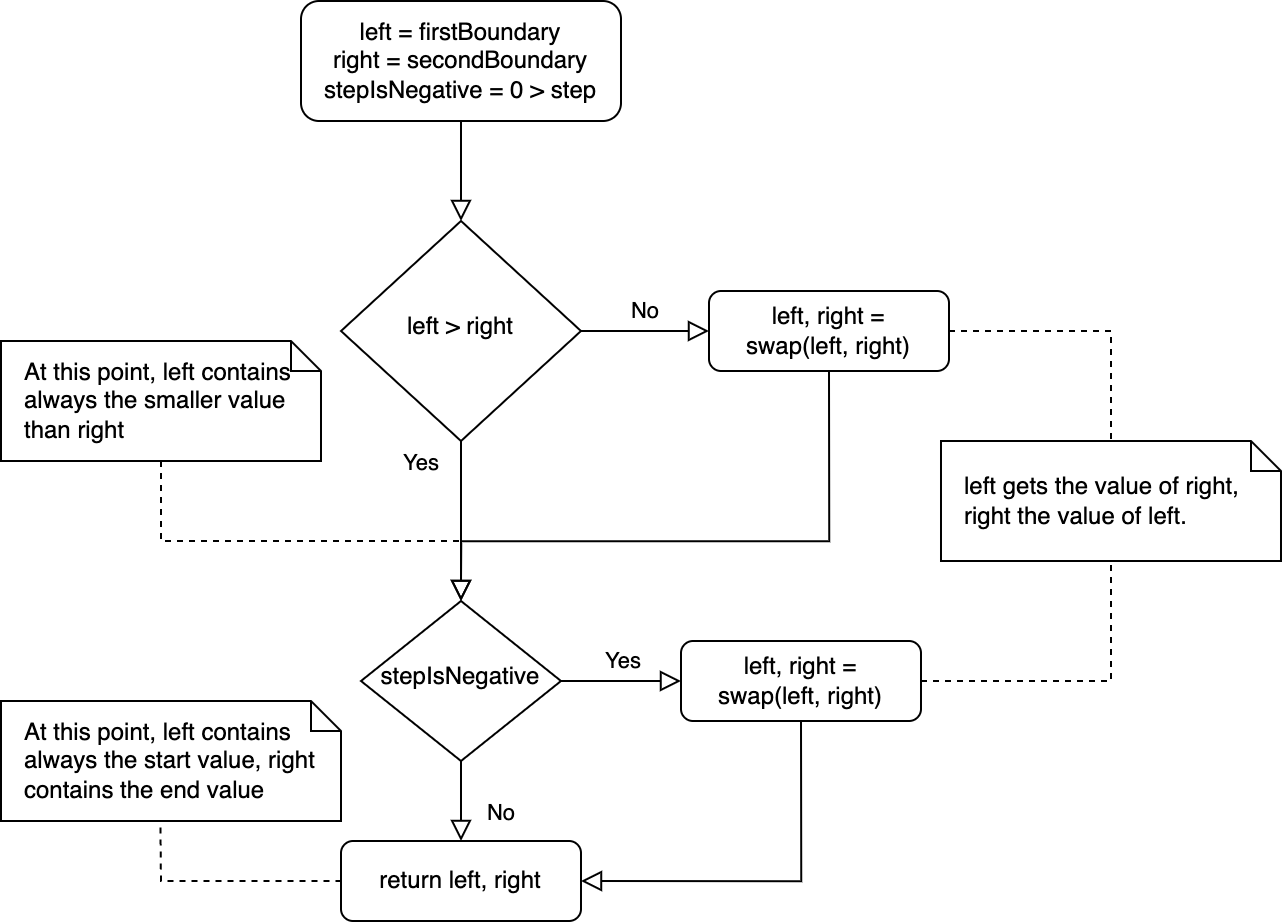
\includegraphics[width=0.9\textwidth]{mainmatter/pictures/boundary-normalization.png}
    \caption{Normalization Flow-Chart diagram}
    \label{fig:norm-flowchart}
\end{figure}

\subsubsection{The End of a Range}
\label{subsub:The End of a Range}
The |hasReachedEnd| function detects the end of the range and defines the
|untilFunction| of the underlying sequence. Listing~\ref{lst:impl_hasReachedEnd}
shows the implementation of the function:

\begin{lstlisting}[
  style=ES6, 
  caption=hasReachedEnd implementation,
  label={lst:impl_hasReachedEnd}
  ]
/**
 * Determines if the end of the range is reached.
 * @param   { Boolean } stepIsNegative
 * @param   { Number }  next - the current element of the range
 * @param   { Number }  end  - the last value of the range
 * @returns { boolean }
 */
const hasReachedEnd = (stepIsNegative, next, end) =>
    stepIsNegative ? next < end : next > end;
\end{lstlisting}

The function must be able to distinguish between two different cases:

\begin{itemize}
  \item If the step size is a negative, the range counts from top to bottom:
    The range reached its end as soon as next is smaller than right.
  \item If the step size is positive, the range counts from bottom to top: The
  range reached its end as soon as next is larger than right.
\end{itemize}

\subsubsection{Some Restrictions of Using a Range}
\label{subsub:Some Restrictions of Using a Range}
When using the range, one has to pay attention to the contract:
\begin{itemize}
\item End value may not be reached exactly, but will never be exceeded.
  \item Zero step size leads to infinite loops, returning always the same values.
  \item Only values that behave correctly with respect to addition and size
    comparison may be passed as arguments.
\end{itemize}


\subsubsection{Using a Range}
\label{subsub:Using a Range}
Following listing~\ref{lst:range_examples} demonstrates various ways to
construct a range.

\begin{lstlisting}[
  style=ES6, 
  caption=Range examples,
  label={lst:range_examples}
  ]
// typical cases
for (const value of Range(3)) { console.log(value); }
// => Logs '0, 1, 2, 3'

for (const value of Range(2,3)) { console.log(value); }
// => Logs '2, 3'

// lower and upper boundaries interchanged
for (const value of Range(3,2,1)) { console.log(value); }
// => Logs '2, 3'

// negative step size
for (const value of Range(4,6,-2)) { console.log(value); }
// => Logs '6, 4'

for (const value of Range(6,4,-2)) { console.log(value); }
// => Logs '6, 4'

// range with negatgive boundary
for (const value of Range(0,-2,-1)) { console.log(value); }
// => Logs '0, -1, -1'
\end{lstlisting}

\section{Iterables Everywhere}
\label{sec:Iterables Everywhere}
The JS iteration protocols are suitable for a wide variety of data structures.
With the sequence library defining many operations for iterables, it makes
sense to make more objects iterable. For example, the Kolibri Web UI toolkit
defines the immutable data structure "pair", for which there are noteworthy
applications if it is iterable. 
\subsection{Making immutable Data Structures iterable}
\label{sub:Making immutable Data Structures iterable}
Listing~\ref{lst:pair_non_iterable} defines the type pair and shows its usage:
\begin{lstlisting}[
  style=ES6, 
  caption=Immutable Pair,
  label={lst:pair_non_iterable}
  ]
/** *'\label{line:start_pair_type}'*
 * @typedef PairType
 * @type {  <_T_, _U_>
 *          (x: _T_)
 *       => (y: _U_)
 *       => (s: PairSelectorType<_T_, _U_>) => ( _T_ | _U_ ) 
 *      }
 */ *'\label{line:end_pair_type}'*
const Pair = x => y => selector => selector(x)(y);

const pair = Pair(1)(2);

const one  = pair(fst);*'\label{line:fst_pair}'*
const two  = pair(snd);*'\label{line:snd_pair}'*

console.log(one + " " + two);
// => Logs '1 2'
\end{lstlisting}

The only way to make a pair immutable is to build it using functions. The type 
signature on line~\ref{line:start_pair_type}~-~\ref{line:end_pair_type} shows 
that the first two arguments are arbitrary values. Pair stores these two values
in its closure scope, the only scope in JavaScript which can not be changed in
any way from the outside.
Selector functions named |fst| on line~\ref{line:fst_pair} and |snd| on 
line~\ref{line:snd_pair} grant access to these values. However, pair offers
no way to modify these values. Listing~\ref{lst:pair_non_iterable} shows that
handling a pair can be tedious. It would be great to use the built-in
JavaScript language features to access the content of a pair.

\subsubsection{Iterable Pair}
\label{subsub:Iterable Pair}
Listing~\ref{lst:pair_iterable} demonstrates the implementation of an iterable 
pair. Still, pair operates only with functions. However, it additionally defines the
|[Symbol.iterator]| property:

\begin{lstlisting}[
  style=ES6, 
  caption=Iterable Pair,
  label={lst:pair_iterable}
  ]
const Pair = x => y => {
  /**
   * @template _T_, _U_
   * @type { PairSelectorType<_T_,_U_> }
   */
  const pair = selector => selector(x)(y);

  pair[Symbol.iterator] = () => [x,y][Symbol.iterator]();*'\label{line:pair_symbol_iterator}'*

  return pair;
};
\end{lstlisting}

Line~\ref{line:pair_symbol_iterator} shows that 
this property defines a function, which only returns the |[Symbol.iterator]|
property of array. The array stores the values of the pair. With that, pairs
are now iterable. Listing~\ref{lst:handling_pair_iterable} shows the usage of
such an iterable pair. Line~\ref{line:pair_destructuring} shows the
deconstruction of a pair in the same way as an array. This access option is
more convenient than in listing~\ref{lst:pair_non_iterable}.
Line~\ref{line:show_pair} demonstrates the usage of operations from the Sequence
library alongside a pair. |show| converts an iterable into a string, analogous
to how |toString| works.

\begin{lstlisting}[
  style=ES6, 
  caption=Working with iterable Pairs,
  label={lst:handling_pair_iterable}
  ]
const pair = Pair(1)(2);

const [one, two] = pair;*'\label{line:pair_destructuring}'*

console.log(show(pair));*'\label{line:show_pair}'*
// => Logs '[1,2]'
\end{lstlisting}

This has significant advantages because it is now possible to process different 
collections with the same abstractions. Therefore, the motivation is great to 
make all collections iterable.

% chapter Iterators in JavaScript (end)

\section{Gluing Programs together}
John Hughes says functional programming languages provide two extra ways to
better partition programs and easily hang them together later. He refers to
this as "glue". These "glues" are on the one hand higher order functions and on
the other hand lazy evaluation. \cite{hughes_why_1989}

\subsection{Using these Glues in Haskell} % (fold)
\label{sub:Using these Glues in Haskel}

\subsubsection{Higher Order Functions in Haskell} % (fold)
\label{sec:Higher order functions Haskell}
Higher order functions are functions that receive another function as arguments
or produce a function as a result. In Haskell, where the whole program is
actually a single function, this concept is of course particularly strong.
The easiest way to understand higher order functions is to look at an
example:

\begin{lstlisting}[style=Haskell, caption=Higher order functions in
Haskell \label{lst:hof_haskell}]
double    = \x -> 2 * x
quadruple = \x -> 4 * x
doubles   = map double [1,2,3,4]
quads     = map quadruple [1,2,3,4]

print $ doubles ++ quads
-- Prints '[2,4,6,8,4,8,12,16]'
\end{lstlisting}

Listing~\ref{lst:hof_haskell} shows how higher order functions work in Haskell.
Code can easily be reused this way, since |map| can be parametrized with a
function.
% subsubsection Higher order functions Haskell (end)

\subsubsection{Lazy evaluation} % (fold)
\label{subsub:Evaluation}
Lazy evaluation means that only as many program statements are evaluated as are
actually required. This makes it possible to work with lists that have an
infinite amount of values. This can best be shown in an example as well.

\begin{lstlisting}[
  style=Haskell,
  caption=lazy evaluation in Haskell,
  label={lst:lazy_eval_haskell}
]
as = [1..]*'\label{line:lazy_eval_haskell_1}'*
doubles = map double as*'\label{line:lazy_eval_haskell_2}'*

print $ take 4 doubles 
-- Prints '[2,4,6,8]'
\end{lstlisting}

Line~\ref{line:lazy_eval_haskell_1} in Listing~\ref{lst:lazy_eval_haskell}
defines a list with infinite values is created. Then the function |double|
defined in Listing~\ref{lst:hof_haskell}, is applied on this list. Since the
list has an infinite amount of elements this would take forever. But since
Haskell evaluates its statements lazy, Nothing happens on
line~\ref{line:lazy_eval_haskell_2}. The |double| function is only applied when
the elements are actually used. This is only the case when they are printed
with |print|. With |take| the list is reduced to four elements. The function
|double| is then only applied to these four elements. \\ More theoretically,
when the function |f| is applied to |g x|, |g| produces only as much output as
|f| actually needs. Therefore, working with a big amount data becomes much more
convenient and faster as well. If the elements in a list are generated with a
rule (as with list comprehensions), lazy evaluation brings great advantages:
The whole list will never materialize in the memory, but only the current
value. So you don't have to worry about what happens when large amounts of data
are processed. \\ Using these two concepts, it is much easier to build large
programs consisting of small parts.
% subsubsection Lazy evaluation (end)
% subsection Using the glues in Haskell (end)

\subsection{Using these Glues in JavaScript} % (fold)
\label{sub:Using these Glues in JavaScript}

\subsubsection{Higher Order Functions in JavaScript} % (fold)
\label{subsub:Higher Order Functions in JavaScript}
Higher order functions in JavaScript work similarly as they to in Haskell. \\
So the meaning of the Listing~\ref{lst:hof_haskell} can be translated to 
JavaScript like:

\begin{lstlisting}[
  style=ES6,
  caption=Higher order functions in JavaScript,
  label={lst:hof_in_js}
]
const double    = x => 2 * x;
const quadruple = x => 4 * x;
const doubles   = [1,2,3,4].map(double);
const quads     = [1,2,3,4].map(quadruple);

console.log(doubles.concat(quads));
// => Logs '2, 4, 6, 8, 4, 8, 12, 16'
\end{lstlisting}
% subsubsection Higher Order Functions in JavaScript (end)

\subsubsection{Eager Evaluation in JavaScript} % (fold)
\label{subsub:Eager Evaluation in JavaScript}

% subsubsection Lazy Evaluation in JavaScript (end)
When it comes to lazy evaluation in JavaScript, it becomes less intuitive:
JavaScript does not know this concept when working with its in-built arrays.
Mapping over an array producing a side effect can shed some light on this:

\begin{lstlisting}[
  style=ES6,
  caption=JavaScript evaluates eagerly,
  label={lst:js_eagerly_eval}
]
const as     = [1,2,3,4,5];
const bs     = [];
const mapped = as.map(x => {
  bs.push(x);
  return 2*x;
});

console.log(mapped.slice(0,4));
// => Logs '2, 4, 6, 8'
console.log(bs);
// => Logs '2, 4, 6, 8, 10'
\end{lstlisting}

Through Listing~\ref{lst:js_eagerly_eval} it becomes clear, that although only
the first four elements of the array are actually used, each element of the
array is still traversed using the |map| function. This can be seen from the
fact that the array |bs| contains all elements of the array |as| and not just
the first four.

\subsubsection{Lazy Evaluate Iterables} % (fold)
\label{Lazy Evaluate Iterables}

% subsubsection Lazy Evaluate Iterables (end)
The eager evaluation of JavaScript is a significant limitation when working with it.
Fortunately, JavaScript provides a way to emulate this laziness using the
Iterable protocols, which the section~\ref{sec:Sequence and Iterable in General}
describes. \\ 

With the use of the sequence library, it is possible to rewrite the JS Code of
Listing~\ref{lst:js_eagerly_eval} lazily:


\begin{lstlisting}[
  style=ES6,
  caption=Lazy evaluation in JavaScript,
  label={lst:lazy_eval_js}
]
const as     = [1,2,3,4,5];
const bs     = [];
const mapped = map(x => {
  bs.push(x);
  return 2*x;
})(as);

console.log(...take(4)(mapped));
// => Logs '2, 4, 6, 8'
console.log(bs);
// => Logs '2, 4, 6, 8'
\end{lstlisting}

The first output is the same as in Listing~\ref{lst:js_eagerly_eval} - the
first four elements of the array |as| have been multiplied by 2. However, the
second output differs: the array |bs| now contains only four elements. So the
function passed to |map| was only applied to four elements of the initial
array! This proves that arrays are processed lazily when transformed using the
Sequence Library!\\
This works because the iterable protocols process element by element. The
iterator delivers the next element only if it is requested. If no further
element is needed, you just don't ask the iterator for the next element! This
decouples the termination condition (asking the iterator for another element)
from the loop body (how the iterator generates/accesses the next element).\\

Furthermore, it is even possible to port the initial Haskell laziness
example defined in Listing~\ref{lst:lazy_eval_haskell} to JavaScript:
\begin{lstlisting}[
  style=ES6,
  caption=Process infinite sequences in JavaScript,
  label={lst:inf_seq_js}
]
const seq = Sequence(1, _ => true, x => x + 1);*'\label{line:inf_seq_js_1}'*
const doubles = map(double)(seq);

console.log(...take(4)(doubles));
// => Logs '2, 4, 6, 8'
\end{lstlisting}

If the code displayed in Listing~\ref{lst:inf_seq_js} were evaluated eagerly,
this would go on forever since line~\ref{line:inf_seq_js_1} defines a sequence
with infinite elements. \\ 

\subsubsection{Placing the Receiver at the End} % (fold)
\label{subsub:Placing the Receiver at the End}
Compared to object-oriented programming languages, where the receiver of an
operation is always placed before the point (i.e., at the beginning), functions
in Haskell usually expect it as the last argument. If one sticks to this, it is
possible to build a new function from a pre-configured function in Haskell
(line~\ref{line:precon_fs_hs_1} of Listing~\ref{lst:precon_fs_hs}) and then
reuse these this function:

\begin{lstlisting}[
  style=Haskell,
  caption=Pre-configured functions in Haskell,
  label={lst:precon_fs_hs}
]
double    = \x -> 2 * x
doubleAll = map double --*'\label{line:precon_fs_hs_1}'* preconfigure map with the function double
as        = [1,2,3,4]
bs        = [5,6,7,8]

print $ doubleAll as ++ doubleAll bs
-- Prints '[2,4,6,8,10,12,14,16]'
\end{lstlisting}

This paradigm allows it also to link existing functions together using the |.|
operator:

\begin{lstlisting}[
  style=Haskell,
  caption=Function composition in Haskell,
  label={lst:fn_comp_hs}
]
-- "sum" sums up all elements in the list
doubleAndSum = sum . doubleAll

print $ doubleAndSum [1,2,3,4]
-- Prints '20'
\end{lstlisting}

The Listing~\ref{lst:fn_comp_hs} links the function |doubleAll| defined in
Listing~\ref{lst:precon_fs_hs} and the function |sum| to create a new function
applicable to any list with numerical values. This concept makes the code very
reusable.\\
Placing the receiver at the end is another powerful modularization
tool. Therefore, the sequence library supports this kind of modularization.
Let us refactor the initial example from Listing~\ref{lst:hof_in_js}, which 
shows how higher-order functions work in JavaScript:
\begin{lstlisting}[
  style=ES6,
  caption=Receiver before the point,
  label={lst:rec_bef_point}
]
// initial code
const double  = x => 2 * x;
const doubles = [1,2,3,4].map(double);

// refactored using plain JS
const doubleAll = receiver => receiver.map(double);
console.log(doubleAll([1, 2, 3, 4]));
// => Logs '2, 4, 6, 8'
\end{lstlisting}

The Listing~\ref{lst:rec_bef_point} shows that this could be fixed using a
function which gets the receiver as an argument. However, this is not very
convenient. The sequence library provides a more elegant way to solve this:

\begin{lstlisting}[
  style=ES6,
  caption=Place the receiver at the end in JavaScript,
  label={lst:rcv_at_end_js}
]
const doubleAll = map(double);
\end{lstlisting}

The code in Listing~\ref{lst:rcv_at_end_js} is not only less to type, but also
more expressive, because the function |map(double)| just gets the new name
|doubleAll|.
% subsubsection Placing the Receiver at the End (end)

\section{Monads in JavaScript} % (fold)
\label{sec:Monads in JavaScript}

\subsection{Wrapping values in a context} % (fold)
\label{sub:Wrapping values in a context}

In Haskell, you often work with values wrapped in a particular context. This
context can be, for example, a list. Nevertheless, this context can also be
another data structure, for example, |Maybe|. \\
For the context |Maybe| two implementations in Haskell co-exist:

% section Monads in JavaScript (end)
\begin{lstlisting}[
  style=Haskell,
  caption=The data type Maybe in Haskell,
  label={lst:maybe_hs}
]
-- defining the datatype Maybe
data Maybe a = Nothing | Just a
\end{lstlisting}

The Listing~\ref{lst:maybe_hs} defines this datatype. Why is this useful?
Imagine you want to create a function |head|, which returns the first value of
a given list. |head| is pretty simple to implement. But wait, what to do when
the list is empty? In object-oriented languages, one might return |null|. The
problem with this solution is that the user must remember that the list can be
empty, and thus the result of |head| can be |null|. This is very error-prone.
\\

That is where the new datatype |Maybe| comes in. |Maybe| allows us to describe
either the absence of a value or the value itself. The following
Listing~\ref{lst:safe_head} defines a new function |safeHead|
(line~\ref{line:safe_head1}), which does
precisely this - it returns |Just a| when the list is not empty
(line~\ref{line:safe_head2}) and |Nothing| otherwise (line~\ref{line:safe_head3}):

\begin{lstlisting}[
  style=Haskell,
  caption=Safely get the first element of a list,
  label={lst:safe_head}
]
-- a function which produces a Maybe:
safeHead :: [a] -> Maybe a *'\label{line:safe_head1}'*
safeHead (a:_) = Just a *'\label{line:safe_head2}'*
safeHead []    = Nothing *'\label{line:safe_head3}'*

printHead list = print $ case (safeHead list) of 
  Just val -> show val
  Nothing  -> "List was empty!"

printHead [1,2,3,4]
-- Prints '"1"'
printHead []
-- Prints '"List was empty!"'
\end{lstlisting}

The difference with returning just |null| is that the user now has to
explicitly deal with the case where there is no first element. This leads to
improved safety.
\subsubsection{Doing the same in JavaScript} % (fold)
\label{subsub:Doing the same in JavaScript}
Listing~\ref{lst:maybe_js} defines the same type in JavaScript:
\begin{lstlisting}[
  style=ES6,
  caption=The data type Maybe in JavaScript,
  label={lst:maybe_js}
]
const Just    = x => _f => g => g(x);*'\label{line:maybe_js1}'*
const Nothing = f => _g => f(undefined);*'\label{line:maybe_js2}'*
\end{lstlisting}

So |Just| and |Nothing| are just functions! How could it be different in
functional programming? \\ 
Line~\ref{line:maybe_js1} defines the |Just| case:
|Just| takes a value |x| and two functions while not using the first function
at all. |Just| applies the second function to the initial value |x|. \\ 
|Nothing| looks very similar to |Just|, with the difference that is does not
receive a value, and the first and not the second function will be called.\\ 

Now how can this be used? Noticeably, |Just(value)| and |Nothing| have the same
structure: both receive two functions as arguments. That means they are
structurally the same. Listing~\ref{lst:js_safeHead} takes advantage of this
property to port the previous function |safeHead| to JavaScript:

\begin{lstlisting}[
  style=ES6,
  caption=safeHead implmented in JavaScript,
  label={lst:js_safeHead}
]
const safeHead = list => {
  const head = list[0];
  return head ? Just(head) : Nothing;
};

const printHead = list => {
  const maybeHead = safeHead(list);
  maybeHead *'\label{line:js_safeHead1}'*
    (_ => console.log("List was empty!")) // Nothing case
    (head => conso.log(head));            // Just case
};

printHead([1,2,3,4]);
// => Logs '1'
printHead([]);
// => Logs 'List was empty!'
\end{lstlisting}

Using the structural similarity of |Just(value)| and |Nothing|,
lines~\ref{line:js_safeHead1} and following evaluate the result of |safeHead|.
% subsubsection Doing the same in JavaScript (end)
% subsection Wrapping values in a context (end)

\subsection{Working with values in a context} % (fold)
\label{sub:Working with values in a context}
\subsubsection{Introducing fmap} % (fold)
\label{subsub:Introducing fmap}
The example with |Maybe| shows how values work in a context. Over time,
however, it can become tedious to keep making this distinction between whether
it has value. Therefore, Haskell offers a concept of working with values in a
context. The simplest way to work with the value using this concept is using
the function |fmap|. |fmap| knows how to execute a function for the value(s) in
a context. Listing~\ref{lst:fmap_maybe_hs} shows the usage of |fmap| for
|Maybe|:

\begin{lstlisting}[
  style=Haskell,
  caption=fmap applied to Maybe,
  label={lst:fmap_maybe_hs}
]
double = (\x -> 2*x)
print $ fmap double (Just 5)
-- Prints 'Just 10' 
print $ fmap double Nothing
--> Prints 'Nothing'
\end{lstlisting}

Similar to |Maybe| also lists describe such a context.
Listing~\ref{lst:hs_fmap_list} shows how |fmap| works on lists:

\begin{lstlisting}[
  style=Haskell,
  caption=fmap applied to a list,
  label={lst:hs_fmap_list}
]
print $ fmap double [1,2,3,4,5]
--> Prints '[2,4,6,8,10]'
\end{lstlisting}

Applying |fmap| to a list has the same result as applying |map| to a list.
Therefore, |fmap| is just a way to "map values".

% subsubsection Introducing fmap (end)
\subsubsection{Making a Context Monadic} % (fold)
\label{sec:Making a Context Monadic}
Haskell defines many other functions analogous to |fmap| to interact with
values in a context. Some of them are more powerful than |fmap|. The following
section gives a brief overview of which operations exist on monads. For a
detailed introduction to this topic, see, for example, ~\cite{monads_adit_2013}. \\

If the context supports the following operations, it is considered monadic:

\begin{itemize}
  \item \textbf{Functor}: A context |f| is a |Functor| when it provides a function
|fmap|. |fmap| receives another function as an argument and applies it to the
value(s) in the context.\\
\item \textbf{Applicative}: A context |f| is an |Applicative| when it is a |Functor|
and additionally provides two functions:
\begin{itemize}
  \item |<*>| (pronounced "app") receives another function as an
    argument wrapped in the same context and applies the unwrapped function to
    the value(s) in the context.
  \item |pure| receives a single argument and wraps it in the context. When
    describing |pure|, people often use the term lifting instead of wrapping.
    |pure| lifts a value into a context.\\
 \\
\end{itemize}
\item \textbf{Monad}: A context |f| is a |Monad| when it is an |Applicative| and
additionally provides a function |>>=| (pronounced "bind"). |>>=| takes another
function as an argument which, when applied to the value(s), again creates a
value in the same context. So that the value(s) are not nested in the context,
|>>=| resolves the inner context again. |>>=| is like |fmap| but after mapping,
the value(s) get flattened. Therefore, this operation is often also referred to
as |flatMap|.
\end{itemize}

Some of these functions have special rules they must follow. Chapter "TODO link
chapter" discusses these rules using their corresponding JavaScript
implementation.
% subsubsection Making a Context Monadic (end)
\subsubsection{Why using these constraints?} % (fold)
\label{sec:Why using these constraints?}
These constraints allow building general functions that can handle various
types. Listing~\ref{lst:hs_why_use_constraints} shows a function |doubleAll|
applicable to |List|s and also |Maybe|s:

\begin{lstlisting}[
  style=Haskell,
  caption=Double the values in a context,
  label={lst:hs_why_use_constraints}
]
doubleAll :: (Functor f) => f Int -> f Int
doubleAll = fmap double

print $ doubleAll [1,2,3,4]
-- Prints '[2,4,6,8]'
print $ doubleAll $ Just 1
-- Prints 'Just 2'
\end{lstlisting}

Even though a |List| and a |Maybe| have nothing in common, the same function
can be applied to both types! \\ 
\textit{Note:} Another example that makes use of this is JINQ, which is described in the
section "TODO link section here".

% subsubsection Why using these constraints? (end)
% subsection Working with values in a context (end)

\subsection{Monads in JavaScript} % (fold)
\label{sub:Monads in JavaScript}
Since monads are so good at handling values in a context, this concept is also
interesting for JavaScript. However, JavaScript has a weaker type system than
Haskell. Therefore, two important concepts can not be transferred to
JavaScript: 
\begin{enumerate}
  \item In Haskell, it is possible, to force the type hierarchy hinted in
    Section~\ref{sec:Making a Context Monadic}.
  \item Haskell can use its type system to determine a specific implementation
    for a function. The Listing~\ref{lst:hs_fn_body} shows the binding of the
    function body to the name using the example of |fmap|:
    \begin{lstlisting}[
      style=Haskell,
      caption=Haskell determines the correct function body,
      label={lst:hs_fn_body}
    ]
-- The implementation for List is used
print $ fmap double [1,2,3,4]
-- The implementation for Maybe is used
print $ fmap double (Just 1)
    \end{lstlisting}
\end{enumerate}


Since it is not possible to implement these two concepts in JavaScript, a
different approach to these two problems is needed:
\begin{enumerate}
  \item Although it is possible to model a type hierarchy in JavaScript,
    enforcing it is impossible. Therefore, we created only one type, the
    |MonadType|. |MonadType| can be used as an interface, which defines all
    operations a monadic type must support.
  \item Instead of type inference and global functions, we added all operations
    to the corresponding object's prototype. \cite{mdn_prototype_2023}
\end{enumerate}

\subsubsection{Which operations fit JavaScript?} % (fold)
\label{Which operations fit JavaScript?}
Since JavaScript works quite differently than Haskell, not all operations are
equally suitable to adopt. \\
The |MonadType| specifies the following operations:
\begin{itemize}
  \item |famp|: Changing values inside a context is a typical pattern,
    also in JavaScript. Porting |fmap| to JavaScript brings many benefits,
    therefore.
  \item |pure|: At first sight |pure| is a function that is not needed.
    However, it quickly became apparent during use that it is often practical
    to lift an element into context via an abstracted function. \\ This is
    often the case when using |>>|.
  \item |>>=|: The |bind| operator allows access to the result of the last
    computation. |Bind| is the only way to determine a new result depending on
    the previous result. \\ Since in JavaScript function names must not contain
    the special characters |>| and |=|, |>>=| cannot be used. |Bind| is also
    already an existing function on every object. Using another term is
    required, therefore. We used the name |and| because it nicely expresses
    that the following result depends on the previous one.
  \item |empty|: The |empty| function creates a context without a value. For
    example, with |Maybe| it is |Nothing| with |List| it is |[]|. A monad does
    not need to provide a function |empty|, so Section~\ref{sec:Making a
    Context Monadic} does not include it. However, |empty| is a function
    available on many monads and is very handy during the programming of
    generic functions. Therefore, the |MonadType| specifies |empty| as well.

\end{itemize}
% subsubsection Which operations fit JavaScript? (end)
\subsubsection{What about the app operator?} % (fold)
\label{sec:Which operations do not fit JavaScript?}
The operator |<*>| is great when applying a function wrapped in a context to
values wrapped in a context. This use-case is relatively rare in JavaScript
because you do not operate as strictly in contexts as in Haskell. In addition,
the app operator also only works on functions that accept their arguments
curried. Most functions in JavaScript do not. Using the JavaScript |Maybe| as
an example, Listing~\ref{lst:app_js_maybe} shows how |<*>| would work:

\begin{lstlisting}[
  style=Es6,
  caption=The app operator in JavaScript used on Maybe,
  label={lst:app_js_maybe}
]
const x = 1, y = 0;
const plus = x => y => x + y; *'\label{line:app_js_maybe1}'*
const jPlus = Just(plus); 
const sum = jPlus.app(Just(x)).app(Just(y)); *'\label{line:app_js_maybe2}'*

sum 
  (_ => console.log("Something went wrong") // Nothing case
  (s => console.log(s));                    // Just case 
// => Logs '1'
\end{lstlisting}

Line~\ref{line:app_js_maybe1} specifies the curried function |plus|. This
function is lifted into the |Maybe| context. Then |<*>| applies the function
|plus| to summand by summand on line~\ref{line:app_js_maybe2}.\\
As this example shows, the usefulness of |<*>| is relatively limited in
JavaScript because functions rarely occur in context. Additionally, |>>=| can
solve everything solvable with |<*>|. \\ 
Listing~\ref{lst:and_js_maybe} shows how |>>| solves the same problem:

\begin{lstlisting}[
  style=ES6,
  caption=The app operator replaced by and,
  label={lst:and_js_maybe}
]
const x = 1, y = 0;
const plus = x => y => x + y; 
const jPlus = Just(plus); 
const sum = jPlus.and(f => f(x)).and(g => g(y)); *'\label{line:and_js_maybe1}'*

sum 
  (_ => console.log("Something went wrong") // Nothing case
  (s => console.log(s));                    // Just case
// => Logs '1'
\end{lstlisting}
Line~\ref{line:and_js_maybe1} shows how |and| gives access to the last element.
Which is the function |plus| the first time and then the function |plus(x)|.

% subsubsection Which operations do not fit JavaScript? (end)
% subsection Monads in JavaScript (end)

\include{./mainmatter/development/naming}
\section{Decorating Sequences}
\label{sec:Decorating Sequences}
This chapter explores how to modify Sequences by implementing the Decorator 
Pattern and effectively managing Sequence state. And then we will discover 
powerful techniques to enhance Sequence functionality and manipulate data.

\subsection{Decorator Pattern}
\label{sub:Decorator Pattern}
Let us look at the Decorator Pattern~\cite[p.~226]{gang_of_four_depa} to understand the content of the 
following sections. In object-oriented programming, the Decorator Pattern is a 
widely used concept. An object decorates another, as the name implies. As a 
result, an outer object holds an inner object, while both implement the same 
interface. The outer object forwards requests to the inner one. This enables
the outer to modify (decorate) the behavior of the inner. 
Figure \ref{fig:seq_diagramm} shows how a decorator forwards the receiving calls and 
transfers the answer back to the client.

% TODO: replace
\begin{figure}[H]
    \centering
    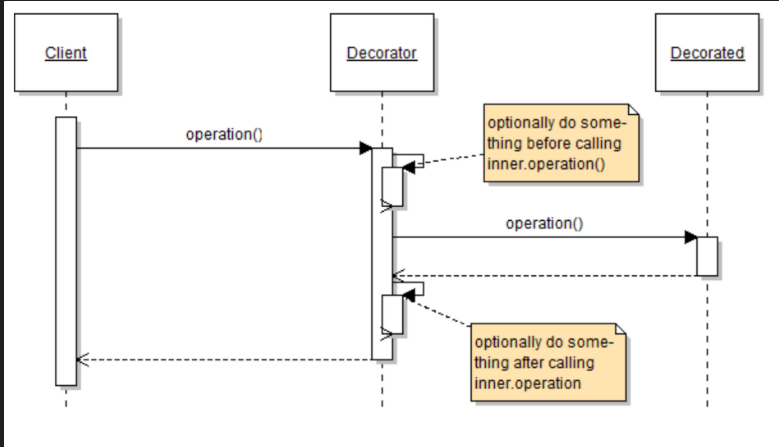
\includegraphics[width=0.8\textwidth]{./mainmatter/pictures/decorator_sequence_diagramm.png}
    \caption{Decorator Patter Sequence Diagram}
    \label{fig:seq_diagramm}
\end{figure}

The Decorator Pattern is often used in object-oriented programming languages 
because of its ability to add functionality to an object at runtime. It is also 
possible to add extended functionality to a single class object. In the 
following, we will see how to exploit this to manipulate and change an Iterable.

\subsection{Processing Sequences}
\label{sec:Processing Sequences}
This section explains how the Sequence Library uses the Decorator pattern.
In the following, the |map| implementation demonstrates the implementation of it. 

\subsubsection{Processing Iteratbles with Functions}
\label{subsub:Processing Iterables with Functions}
In the following, |map| serves as a representative for any function of the
Sequence Library. We call such functions in the following operators,
according to the package they are in.
Listing~\ref{lst:impl_map} shows how |map| processes a Sequence. The
implementation use the Decorator approach just mentioned. |map| decorates a
|Sequence| on line~\ref{line:obj_mapped}.
\newline
On line~\ref{line:args}, the function signature shows that a client can invoke 
|map| with two arguments:

\begin{enumerate}
  \item{A mapper-function capable of processing an element of an |Iterable|}
  \item{An |Iterable|}
\end{enumerate}

An iterable must adhere to the JS iteration protocol 
outlined in Section~\ref{subsub:The Iterable Protocol}. Therefore, |map| can 
process Sequences, Arrays, or any other iterable. 

\begin{lstlisting}[
  style=ES6, 
  caption=Implementation of map,
  label={lst:impl_map}
  ]
const map = mapper => iterable => { *'\label{line:args}'*
*'\label{line:state_iterable}'*
const mapIterator = () => {
   const inner = iteratorOf(iterable);*'\label{line:state_iterator}'*
   let mappedValue;
 
   const next = () => {
     const { done, value } = inner.next();*'\label{line:inner_next}'*
     if (!done) mappedValue = mapper(value);
 
     return { /**@type boolean */ done, value: mappedValue }
   };
 
   return { next };
  };
 
  return createMonadicSequence(mapIterator);
};

const sequence = Sequence(0, x => x < 10, x => x++);*'\label{line:seq_definition}'*
const mapped   = map(x => x * 2)(sequence);*'\label{line:obj_mapped}'*
\end{lstlisting}

Because |map| decorates iterables, |map| also returns an object adhering JS
iteration protocols. 
We define this object on line~\ref{line:obj_mapped} as |mapped|. 
Consequently, |map| also has a next function. Since the JS iteration protocol 
specifies only this single function, it is the only one that must be externally 
callable. The object |mapped| forwards function calls on |next| to the
inner function |next|, on line~\ref{line:inner_next}. The |mapper| function then 
processes the result and returns it. so |map| decorates the function |next| of
the inner |Iterable|.

\subsection{Benefits of the Decorator Approach}
\label{sub:Benefits of the Decorator Approach}
This section discusses the benefits and consequences of using the Decorator 
Pattern to implement the Sequence Library. We start with the fact that functions 
stand-alone, then discuss the options for managing State.

\subsubsection{Stand-alone Functions}
\label{subsub:Standalone Functions}
In an object-oriented approach, the |Sequence| object would provide a function
|map|. Therefore, such operators are available by using dot notation,
similar to Java implements the Stream API \cite{java_stream}. 
However, with the approach of providing independent functions, there 
are three significant advantages:

\begin{enumerate}
  \item {Strict adherence to the open-close principle~\cite[p.~3]{eilebrecht_patterns_2019}. Changes to an operator do
      not affect the implementation of Sequence. Also, extensions to the 
      Sequence Library do not affect existing code.
    }
  \item{Adherence to the single responsibility approach. The Sequence 
      constructor has only the task of creating a sequence. Mapping the
    elements of a sequence is not its responsibility.
  }
  \item{Easy scalability is guaranteed. It is very straightforward to add new 
    functionality from the outside.
  }
\end{enumerate}

Additionally, the |operators| implement their arguments in a curried-style, passing the
receiver at the last position allows the use of eta-reduction in many situations. 
More about this later in the paper.

\subsubsection{Stateful Decorating}
\label{subsub:Stateful Decorating}
A state is present as soon as operators decorate iterables or implement 
additional functionalities. This chapter explores the implementation of state
within operators and the implications it involves.

There are two valid possibilities for including state.
The first Scenario places the state into the closure scope to the surrounding 
operator of the iterator. The second Scenario implements the state into the 
closure scope of the iterator. In both variants, it is crucial to ensure that 
the underlying object remains unchanged.

\subsubsection{Scenario 1}
\label{subsub:Scenario 1}
Listing~\ref{lst:scen_1} shows an example of a Sequence generating numbers from
zero to five. On line ~\ref{line:scen_1_state}, value |i| works as a counter 
and represents the state. 
A call to |SampleIterator| creates a state which is valid for the entire 
object's lifetime.

\begin{lstlisting}[
  style=ES6, 
  caption=Scenario 1 - State in closure scope of iterable,
  label={lst:scen_1}
  ]
const SampleIterable = () => {

  let i = 0; *'\label{line:scen_1_state}'*
  const next = () => {
    return { done: i > 5, value: i++ };
  };

  return { [Symbol.iterator]: () => ({ next }) }
};
\end{lstlisting}

Listing~\ref{lst:scen_1_demo} shows a possible program flow. 
The program first creates an object of |SampleIterator|, maps it and processes
an element on the original object. Note, that on line~\ref{line:scen1_map} |map| also 
uses the same |Iterable|. Line~\ref{line:scen1_output} shows an expected result.

\begin{lstlisting}[
  style=ES6, 
  caption=Scenario 1 - Example usage,
  label={lst:scen_1_demo}
  ]
const seq = SampleIterable(0, x => x < 5, x => x++); // [0, 1, 2, 3, 4]
const mapped = map(id)(seq); *'\label{line:scen1_map}'*

for (const elem of mapped) {
  console.log(elem);
  break; // Just consuming one element
}
// => Logs: '0'

for (const elem of seq) {
  console.log(elem);
}
// => Logs: '[0, 1, 2, 3, 4]' *'\label{line:scen1_output}'*
\end{lstlisting}

To achieve the expected result, |map| must copy the object before processing.
That implies that each |Iterable| must be copyable. An example implementation
of a copyable |Iterable| shows Listing~\ref{lst:iterable_with_copy}.

\begin{lstlisting}[
  style=ES6, 
  caption=Iterable with copy,
  label={lst:iterable_with_copy}
  ]
const SampleIterable = () => {

  let i = 0;
  const next = () => {
    return { done: i > 5, value: i++ };
  };

  const copy = () => SampleIterable();

  return {
    [Symbol.iterator]: () => ({ next }),
    copy: copy *'\label{line:iterable_copy}'*
  }
};
\end{lstlisting}
Since |copy| must be callable from outside, it requires returning it alongside 
|[Symbol.iterator]| on line~\ref{line:iterable_copy} . |map| is now
able to copy the underlying  |Iterable| before consuming the elements.
However, |map| itself must also implement |copy|, because its interface must be
the same as the decorated object. The following Listing~\ref{lst:map_with_copy} 
shows an implementation of |map| supporting copy.

\begin{lstlisting}[
  style=ES6, 
  caption=Implementation of map with copy,
  label={lst:map_with_copy}
  ]
const map = mapper => iterator => {
 const inner = iterator.copy();*'\label{line:copy_of_inner}'*
 let mappedValue;

 const next = () => {
   const { done, value } = inner[Symbol.iterator]().next();*'\label{line:consuming_inner}'*
   if (!done) mappedValue = mapper(value);
   return { done, value: mappedValue }
 };

 return {
   [Symbol.iterator]: () => ({ next }),
   copy: () => map(mapper)(inner*'\label{line:return_copy_map}'* };
};
\end{lstlisting}
On line~\ref{line:copy_of_inner}, |map| references a copy of the original
|Iterable|. Further processing on line~\ref{line:consuming_inner} works on this 
copy to protect the original from being mutated.

In many respects, |copy| is an elaborate thing. All operators and constructors 
dealing with |Iterable|s must implement it. Thus, implementation errors are 
almost certain. On the other hand, it is an extra effort from a performance point 
of view. It means more function calls and also larger stack calls to manage.
The advantage of this implementation is that partially processed iterators can
be further utilized while maintaining their current state, without
reinitializing the state with a new iteration.
Because all objects must have copy implemented, operators can 
only process objects that implement copy. That means JavaScript |array|s or
|HTML Collection| are not processable anymore, which is a significant drawback.

\subsubsection{Scenario 2}
Listing~\ref{lst:scen_2} represents Scenario 2. Here, the state is on
line~\ref{line:scen_2_state} inside the |Iterator|. Running the code from the previous 
example~\ref{lst:scen_1_demo} produces the same output. The distinction lies in
the fact that the object does not need to be copyable. Each call to |[Symbol.iterator]| 
creates a new state. This type of |Iterable| is immutable. Another advantage is
that all operators within the Sequence Library can handle objects conform to JS
iteration protocols including JavaScript |array|s.

\begin{lstlisting}[
  style=ES6, 
  caption=Scenario 2 - State in closure scope of iterator,
  label={lst:scen_2}
  ]
const SampleIterable2 = () => {

  return {
    [Symbol.iterator]: () => {
      let i = 0; *'\label{line:scen_2_state}'*
      return {
        next: () => ({ done: i > 5, value: i++ })
      }
    }
  };
};
\end{lstlisting}

As mentioned in chapter~\ref{sub:Types of Iterables}, there is a reason for 
the deep nesting of the |Iterator|. As you can see now, it serves to make 
the |Iterator| immutable.
\newline
In this chapter, we have examined the possibilities for adding state to 
Sequences. Due to the advantages of immutability, we built the Sequence Library 
according to Scenario 2 with an immutable approach.


\subsection{Adding Monadic Functions to Iterables}
\label{sub:Adding Monadic Functions to Iterables}
In this last section of this chapter, we will highlight one more function we 
have left out so far. It is about the function |createMonadicSequence|, which
can be used to create |Iterable|s.

\subsubsection{A Convenience Function}
\label{subsub:A Convenience Function}
In Section~\ref{subsub:Processing Iterables with Functions}
Listing~\ref{lst:impl_map} shows the implementation of |map|. 
This implementation uses a function |mapIterator|, which returns an object
containing a function |next|. Thus, |mapIterator| forms an |Iterator|.
|createMonadicSequence| now expects such an iterator. As the name suggests, 
|mapIterator| is part of the 
iterable object that follows the JS iteration protocol.
Listing~\ref{lst:createMonadicSequence} demonstrates the implementation of 
|createMonadicSequence|.

\begin{lstlisting}[
  style=ES6, 
  caption=Implementation of createMonadicSequence,
  label={lst:createMonadicSequence}
  ]
/**
 * Builds an {@link SequenceType} from a given {@link Iterator}.
 * @template _T_
 * @param { () => Iterator<_T_> } iterator
 * @returns { SequenceType<_T_> }
 */
 const createMonadicSequence = iterator => {
   *'\label{line:start_createMonadicSequence}'* const result = {[Symbol.iterator]: iterator};
  return setPrototype(result);
};*'\label{line:end_createMonadicSequence}'*


/**
 *
 * @template _T_
 * @param { Iterable<_T_> } iterable
 * @returns { SequenceType<_T_> }
 */
 const setPrototype = iterable => { *'\label{line:setPrototype}'*
  Object.setPrototypeOf(iterable, SequencePrototype);
  return /**@type SequenceType*/ iterable;
};
\end{lstlisting}

Between line~\ref{line:start_createMonadicSequence} and 
line~\ref{line:end_createMonadicSequence}, we can recognize main tasks of the
function |toMonadicSequence|.

\begin{itemize}
  \item{Assign the passed iterator to the |[Symbol.iterator]| property}
  \item{Add the Sequence prototype to the resulting object}
\end{itemize}

Many of the operations of the Sequence Library use this code.
Outsourcing the code helps to improve the code base's overview and readability.
The following section explains what the prototype is all about.

\subsubsection{Sequence Prototype}
\label{Sequence Prototype}
An object in JavaScript can have a prototype. Prototypes define properties 
that are available to the corresponding object. The subsequent
function |setPrototype| on line~\ref{line:setPrototype} sets the Sequence 
prototype to this iterable. This causes some functions to be accessible on each 
|SequenceType| using notation. These are, among others, monadic functions. You will read more
about Monads and there functionality in chapter~\ref{sec:Monads in JavaScript}. 
|SequenceType| represents a Sequence and the monadic functions defined on it. 
Listing~\ref{lst:sequence_type} shows the definition of the type.

\begin{lstlisting}[
  style=ES6, 
  caption=SequenceType definition,
  label={lst:sequence_type}
  ]
/**
 * @template _T_
 * @typedef {
 *  {
 *    and:  <_U_>(bindFn: (_T_)    => SequenceType<_U_>) => SequenceType<_U_>,
 *    pure: <_U_>(_U_)             => SequenceType<_U_>,
 *    fmap: <_U_>(f: (_T_) => _U_) => SequenceType<_U_>,
 *    empty:     ()                => SequenceType<_T_>,
 *    toString:  ()                => String,
 *    "==":      (that:SequenceType<_T_>) => Boolean
 *  } & Iterable<_T_>
 * } SequenceType
 */
\end{lstlisting}

Why is this necessary? With this approach, we can ensure that Sequences become
monadic but still iterable. Monadic APIs can thus also process Sequences. An
example of this is JINQ. Chapter~\ref{TODO} discusses JINQ in detail.


\subsubsection{Turn Iterables into SequenceType}
\label{subsub:Turn Iterables into SequenceType}
Sometimes the |SequenceType| must be set on an arbitrary |Iterable|. For example,
if you want to use the monadic functions on a JavaScript array. To make this
possible, Sequence Library provides |toMonadicIterable| function.
Listing~\ref{lst:casting_iterables} shows the
implementation of it. This function takes an arbitrary |Iterable| and returns an
|SequenceType| mapped by |id| \footnote{The id (identity) function always
returns the value passed to it.}. 
Therefore, the returning object is then of the desired type |SequenceType|.

\begin{lstlisting}[
  style=ES6, 
  caption=Casting an arbitrary Iterable to SequenceType,
  label={lst:casting_iterables}
  ]
/**
 * Casts an arbitrary {@link Iterable} into the {@link SequenceType}.
 * @template _T_
 * @param { Iterable<_T_> } iterable
 * @return { SequenceType<_T_> }
 */
const toMonadicIterable = iterable => map(id)(iterable);
\end{lstlisting}

\section{Experiments}


\section{Introduction}

\section{More Monads}

\section{Prototype Functions}

\section{Iterator Builder}

\section{Query different Data Structures}
\label{sec:Query different Data Structures}
Based on the knowledge from section~\ref{chap:Monads in JavaScript}, other
possibilities analogous to |keepEven| become realizable - i.e., functions that
handle arbitrary monadic structures. \\ 
This section introduces such a concept called Language Integrated Queries
(LINQ), which queries any monadic data structure. It goes into detail
about the implementation of LINQ in JavaScript and shows how you can easily
browse lists of JavaScript objects using LINQ.
\subsection{Introduction to LINQ} % (fold)
\label{sub:Introduction to LINQ}
Some programming languages offer uniform ways to query different data
structures in an SQL-like syntax.

C\# calls this concept LINQ (Language Integrated Query). LINQ allows to
decarlatively query compatible data sources. Listing~\ref{lst:linq_in_csharp}
shows how to use LINQ to query a simple array of numeric values.

\begin{lstlisting}[
  style=sharpc,
  caption=LINQ in C\# \cite{billwagner_language-integrated_2023},
  label={lst:linq_in_csharp}
]
// Specify the data source.
int[] scores = { 97, 92, 81, 60 }; *'\label{line:linq_in_csharp1}'*

// Define the query expression.
IEnumerable<int> scoreQuery =
    from score in scores
    where score > 80
    select score;

// Execute the query.
foreach (int i in scoreQuery)
{
    Console.Write(i + " ");
}

// Output: 97 92 81
\end{lstlisting}

You can replace the data structure defined on line~\ref{line:linq_in_csharp1}
with any other one compatible with this API. This abstraction makes it very
easy to define reusable queries.


% subsection Introduction to LINQ (end)
\subsection{Why does this not exist in JavaScript?} % (fold)
\label{sub:Why does this not exist in JavaScript?}
However, JavaScript does not define a uniform API for data structures except
for the JS iteration protocols and thus cannot offer language-integrated queries
without further effort. \\
Section~\ref{sub:Making the Sequence Monadic} introduced the monadic sequence,
which provides additional operations to work with a sequence. All of these
operations are available through the sequence prototype. Since these
operations work solely on the committed properties of the JS iteration
protocols, the function |toMonadicIterable|, explained in
Section~\ref{sec:Iterables Everywhere} can quickly turn them into a monadic
sequence.\\
With that, a more extensive API is now available to every data structure
conforming to the JS iteration protocols. This monadic API makes it possible to
implement abstractions similar to LINQ in JavaScript.
% subsection Why does this not exist in JavaScript? (end)

\subsection{Introducing JINQ} % (fold)
\label{sub:Introducing JINQ}
JINQ (JavaScript integrated query) is the implementation of LINQ for
JavaScript. It can handle any data that conforms to the |MonadType| explained
in Section~\ref{subsub:The MonadType}. So JINQ can handle monadic iterables and
every monadic type, such as the type |Maybe| introduced in
Section~\ref{sub:Doing the same in JavaScript}.\\
\textit{Note:} All operations supported by JINQ are explained in detail in 
Section~\ref{sec:API_JINQ}. This sections descibres how JINQ works
internally.

Listing~\ref{lst:keepeven_recap} shows again the function |keepEven| already
introduced in Section~\ref{subsub:The MonadType}, which works on a |Maybe| as
well as on a |Sequence|:
\begin{lstlisting}[
  style=ES6,
  caption=Recapitulate keepEven,
  label={lst:keepeven_recap}
]
const keepEven = monad => monad
  .and(x => {
    if (x % 2 === 0) {
      return monad.pure(x);
    } else {
      return monad.empty();
    }
}); 
\end{lstlisting}

JINQ makes it possible to simplify the implementation of this function.
Listing~\ref{lst:keepeven_jinq} therefore introduces a new function
|keepEvenJINQ|, which does precisely the same as |keepEven|:

\begin{lstlisting}[
  style=ES6,
  caption=keepEvenJINQ does the same as keepEven,
  label={lst:keepeven_jinq}
]
const keepEvenJINQ = monad =>
  from(monad)
    .where(x => x % 2 === 0)
    .result();
\end{lstlisting}

|keepEvenJINQ| is not only shorter but also more readable! It becomes clear
within moments what this function does, as it reads almost like prose!\\
This is the power of these abstractions - types must only follow a
minimal API to be compatible with JINQ. Additionally, they are very readable.

\textit{Note:} As explained before, JINQ works only on the monadic API. So you
can just as well use the monadic functions to achieve the same. However, the
example |keepEven| shows that it is easier to work with JINQ and save lines of
code.

\subsubsection{How does JINQ work?} % (fold)
\label{subsub:How does JINQ work?}
JINQ uses a pattern analogue to the Builder pattern
\cite[Chapter~3.2]{gang_of_four_depa} to create a new structure which can be
used to transform the initially passed monad. \\
Have a look at the function on line~\ref{line:jinq_impl1} of
Listing~\ref{lst:jinq_impl}: If |from| is called, a new builder is created.
|from| expects a monad, which serves as the starting point of the builder. The
next operation executed on the builder operates on this monad. |result| then
returns the monad created based on the builder.

\textit{Note:} None of the functions change the parameter |monad| - therefore,
JINQ is immutable! This allows reusing an intermediate state of the JINQ
builder!

\begin{lstlisting}[
  style=ES6,
  caption=How is where implemented?,
  label={lst:jinq_impl}
]
// jinq.js
export { from }
const jinq = monad => ({ *'\label{line:jinq_impl1}'*
  pairWith: pairWith(monad),
  where:    where   (monad),
  select:   select  (monad),
  map:      select  (monad),
  inside:   inside  (monad),
  result:   () =>    monad
});

const from = jinq;*'\label{line:jinq_impl2}'*

// ...
\end{lstlisting}

Listing~\ref{lst:jinq_where_impl} uses the already familiar function |where| to
showcase how the builder operations work:

\begin{lstlisting}[
  style=ES6,
  caption=How is where implemented?,
  label={lst:jinq_where_impl}
]
// jinq.js
// ...

const where = monad => predicate => {
  const processed = 
    monad.and(a => predicate(a) ? monad.pure(a) : monad.empty()); *'\label{line:jinq_where_impl1}'*
  return jinq(processed);*'\label{line:jinq_where_impl2}'*
};

// ...
\end{lstlisting}

You may have already guessed it - the implementation of |where| is almost
precisely the implementation of |keepEven|! It is more general because the
predicate |x % 2 === 0| is outsourced to a function called |predicate|. See
line~\ref{line:jinq_where_impl1} in Listing~\ref{lst:jinq_where_impl}: |and|
keeps a value matching the predicate using |monad.pure| or discards it
otherwise using |monad.empty|.\\
Line~\ref{line:jinq_where_impl2} then wraps the resulting monad in a new
builder instance and returns it.

Another notable function of JINQ is |pairWith| - its implementation is shown in
Listing~\ref{lst:jinq_pairwith_impl}. Use it to combine a data source with
another one (or even with itself):

\begin{lstlisting}[
  style=ES6,
  caption=How is pairWith implemented?,
  label={lst:jinq_pairwith_impl}
]
// jinq.js
// ...

cconst pairWith = monad1 => monad2 => {
  const processed = monad1.and(x =>
    monad2.fmap(y => Pair(x)(y))
  );

  return jinq(processed)
};
// ...
\end{lstlisting}

|pairWith| takes a second monad. It now forms a new monad with a |Pair| in it!
But what happens here? Difficult to say because we can not know it! It just
calls |and| on |monad1| and combines it with |monad2|. \\
So when combining two sequences, every element of the first sequence gets
paired up with every element of the second sequence. One could argue that this
will take too much memory and could be more efficient. But let us step back and
think about Section 2.3, which discusses the laziness of sequences. |monad1|
(a sequence in the current example) is evaluated lazily! So never all
combinations will be materialized in memory at once!
% subsubsection How does JINQ work? (end)

\subsubsection{Creating Sequences using JINQ} % (fold)
\label{subsub:Creating Sequences using JINQ}
A list comprehension in Haskell is an expression form that allows generating
lists in a declarative way. See \cite[Chapter 5]{hutton_pih_2016} for an
in depth introduction to list comprehensions. \\
Listing~\ref{lst:list_comp_hs} creates a list using a list comprehension in
Haskell:

\begin{lstlisting}[
  style=Haskell,
  caption=List comprehension in Haskell,
  label={lst:list_comp_hs}
]
pairs = [(i,j) |        -- create a list of pairs where
          i <- [1..10], -- i can have the values 1 to 10
          j <- [1..4],  -- j can have the values 1 to 4
          i - j == 1]   -- only keep pairs with i - j == 1

print pairs
-- Prints '[(2,1),(3,2),(4,3),(5,4)]'
\end{lstlisting}

Using JINQ, it is possible to create sequences similarly:
\begin{lstlisting}[
  style=ES6,
  caption=Creating Sequences using JINQ,
  label={lst:list_comp_js}
]
const pairs =
  from(Range(1,10))                 // create a seq with values 1 to 10
    .pairWith(Range(1, 4))          // union with a seq containing 1 to 4
    .where(([i, j]) => i - j === 1) // only keep pairs with i - j == 1
    .result();

console.log(pairs.fmap(show).toString());
// => Logs '[[2,1],[3,2],[4,3],[5,4]]'
\end{lstlisting}

Of course, list comprehensions in Haskell provide more syntacitcal sugar than
JINQ. Nevertheless, JINQ provides an easy way to create sequences based on
rules, coming quite close to a list comprehension.
% subsubsection Creating Sequences using JINQ (end)

\subsubsection{Using the JSONMonad to process lists of JavaScript objects} % (fold)
\label{subsub:Using the JSONMonad to process lists of JavaScript objects}
The |JSONMonad| provides arrays of JavaScript objects with a monadic API. The
|JSONMonad| makes them, therefore, compatible with JINQ. This is especially
useful when JavaScript Objects are created from JSON because they often have
missing or nullable fields. The monadic operations of |JSONMonad| deal with
that and ensure that querying nullable attributes do not cause problems.

The Listing~\ref{lst:jsonmonad_data} dives right into an example defining two
records that are related to each other. The first one contains data about an
ancient battle, while the second one contains data about the heroes of the
battle. The |heroId| connects these two records. The battle had a |winner| and
a |loser|. Imagine you want to find all names of the heroes of the winner team.

\begin{lstlisting}[
  style=ES6,
  caption=Two data sources,
  label={lst:jsonmonad_data}
]
const battleData = JSON.parse(`
  {
    "battleName": "The battle of Curly",
    "numberOfDeaths": 420000,
    "winner": { "teamName": "JSON", "outStandingHeroes": [1] },
    "loser": { "teamName": "XML", "outStandingHeroes": [] }
  }
`);

const heroes = JSON.parse(`
  [
    { "heroId": 1, "kills": 47076, "name": "Atonadias" },
    { "heroId": 2, "kills": 5691,  "name": "Tanobiri" },
    { "heroId": 3, "kills": 3707,  "name": "Tonadri" }
  ]
`);
\end{lstlisting}

Listing~\ref{lst:jsonmonad_example} combines these two data sources using JINQ.
Line~\ref{line:jsonmonad_example1} wraps the |battleData| with the |JSONMonad|
to become queriable. |select| then accesses the property |winner| and from
there the property |outstandingHeroes|. Line~\ref{line:jsonmonad_example2}
pairs the second data source before Line~\ref{line:jsonmonad_example3}, then
destructures the |Pair| and only keeps the heroes (from the second data source)
that belong to the winning team (from the first data source).

\begin{lstlisting}[
  style=ES6,
  caption=Combining data sources using JINQ and JSONMonad,
  label={lst:jsonmonad_example}
]
const outstandingHeroNames =
  from(JsonMonad(battleData)) *'\label{line:jsonmonad_example1}'*
    .select   (x => x["winner"])
    .select   (x => x["outStandingHeroes"])
    .pairWith (JsonMonad(heroes)) *'\label{line:jsonmonad_example2}'*
    .where    (([heroId, hero]) => heroId === hero["heroId"]) *'\label{line:jsonmonad_example3}'*
    .select   (([_, hero]) => hero["name"])
    .result   ();

console.log(...outstandingHeroNames);
// => Los 'Atonadias'
\end{lstlisting}

% subsubsection Using the JSONMonad to process lists of JavaScript objects (end)
\subsubsection{Conclusion} % (fold)
\label{subsub:JINQ_Conclusion}
Monadic APIs allow the building of very general abstractions that can handle a
wide variety of data types, even if they seem to have nothing in common at
first glance - such as a sequence or a Maybe! JINQ showcases an excellent
instance of such a general abstraction - its operations only compose generic
monadic functions. Nevertheless, JINQs operations have very expressive names
describing their purpose, making it easy to use JINQ with different data types!
That is truly beautiful and quite rare: general concepts with specific
names!\\ 
JINQ shows its versatility through the possibility of creating new lists based
on declarative rules and using the |JSONMonad|.
% subsubsection Conclusion (end)
% subsection Introducing JINQ (end)
% section Why does this not exist in JavaScript? (end)

\section{How to test}

\section{How to Extend the Library}
\label{sec:How to Extend the Library}
This Chapter gives a quick start to extending the Sequence library. Because
applications are versatile, you may want to add further functionality to the
Library. Therefore, this Chapter explains the relevant steps to simplify the entry.
\newline
Whether you want to add a constructor, an operator, or a terminal operation is
similar. Below is an example of an operator. You can adapt the procedure for
the others.

\subsection{Adding a new Operator}
\label{sub:Adding a new Operator}
In this scenario, we include |concat| to the Sequence library. |concat| is the
operation that appends one |Iterable| to another.

\subsubsection{Kind of the Operation}
The library distinguishes between operators and terminal operations. The
difference depends on the return type. If a function returns an |Iterable|, it
is an operator. It is a terminal operation if it produces a different type than an
|Iterable|, such as |isEmpty|.
Since |concat| returns an |Iterable|, we include the related files into the
operations folder.

\subsubsection{Directory Structure}
\label{subsub:Directory Structure}
|concat| has its folder in the operations directory. Therefore, we create a
|concat.js| and a |concatTest.js| file in the folder |concat|. The reasoning for 
splitting tests into a separate file is that it leads to a better overview and faster
navigation between the particular functionalities. Figure~\ref{fig:concat_dir}
shows the relevant directories.

\begin{figure}[H]
\dirtree{%
  .1 src .
  .2 sequence .
  .3 operators .
  .4 concat .
  .5 concat.js .
  .5 concatTest.js .
  .4 \ldots .
  .4 operators.js .
  .4 operatorsTest.js .
  .3 \ldots .
  .2 AllTests.html .
  .2 \ldots .
  }
  \caption{concat directory structure}
  \label{fig:concat_dir}
\end{figure}

\subsubsection{Exports and Imports}
All artifacts of the Sequence library are available via the |sequence.js| file.
To make |concat| support this, we export it via the |operators.js| file.
Listings~\ref{lst:concat_export} and \ref{lst:concat_export_operators} shows the corresponding statements.

\begin{lstlisting}[
  style=ES6, 
  caption=Export of concat,
  label={lst:concat_export}
  ]
// concat.js

export { concat }
\end{lstlisting}



\begin{lstlisting}[
  style=ES6, 
  caption=Export of concat in operators.js,
  label={lst:concat_export_operators}
  ]
// operators.js
...
export * from "./concat/concat.js"
\end{lstlisting}

The same principle applies to the test files. Importing the |concatTest.js| in
|operatorsTest.js| enables to run of the test cases.

\begin{lstlisting}[
  style=ES6, 
  caption=Export of concat in operatorTest.js,
  label={lst:concat_import_operators}
  ]
// operatorsTest.js
...
import "./concat/concat.js"
\end{lstlisting}

\subsection{Implementing a new Operator}
\label{subsub:Implementing a new Operator}
Now we're getting down to the nitty-gritty.
Because great software engineers start with the tests, we do that first.

\subsubsection{Write the Tests}
\label{subsub:Write the Tests}
Chapter~\ref{sec:Testing} has already explained testing in detail. Therefore, we will only deal 
with the practical part here.
\newline
Let us start with the imports. For testing reasons, we need the following
functionalities:

\begin{itemize}
  \item{TestSuite}
  \item{addToTestingTable}
  \item{createTestConfig}
\end{itemize}

\textit{Note:} You may need additional imports to implement the tests itself.
\newline
Now you are ready to create a test config and, optionally, some special cases.
Creating a test config requires the following steps:

\begin{itemize}
  \item{Create a |TestSuite| with a meaningful name corresponding to the function you are implementing.}
  \item{|createTestConfig| expects an object of type |SequenceTestConfigType|. Have a look
    to this type or to Chapter~\ref{subsub:The Configuration} to get the information about the available properties. }
      \item{If neccessary, add some further test cases using the same TestSuite.}
  \item{Run the |TestSuite| by calling the |run()| function at the end of the file. }
\end{itemize}

Listing~\ref{lst:concat_test_import} shows a scaffold of a test file. 

\begin{lstlisting}[
  style=ES6, 
  caption=Imports of concatTest.js,
  label={lst:concat_test_import}
  ]
import { addToTestingTable }  from "./src/sequence/util/testingTable.js";
import { TestSuite }          from "./src/sequence/test/test.js";
import { createTestConfig }   from "./src/sequence/util/testUtil.js";
import { concat }             from "./src/sequence/sequence.js";
...

const testSuite = TestSuite("Name of the TestSuite");

addToTestingTable(testSuite)(
  createTestConfig({
      ...
    })
);

testSuite.add("test special case", assert => {
  // Given
  ...
  // When
  ...
  // Then
  ...
});

testSuite.run();
\end{lstlisting}

Run the |AllTests.html| file, and you should see that your tests are failing.
If so, then everything is fine.

\textit{Note:} While running the tests, always observe the console.

\subsubsection{Write the Functionality}
Now you are in a comfortable position to implement the function against tests.
For this, we create a function |concat| in the file |concat.js|.
Probably, you can use existing functionalities of the Sequence library to implement them. A list of all
provided functionality is in Chapter~\ref{sub:api_Constructors} - \ref{sub:api_Terminal Operations}.
\newline
Again, run the tests and be proud if everything is running!

\section{Range}

\section{Constructors} % (fold)
\label{sec:api_constructors}
A constructor is anything that builds a |Sequence| without depending on another
one. So they serve as an entry point to the Sequence library. Some of these
constructors create a specific series of values, including, for example, the
|PrimeNumberSequence| which yields the infinite sequence of all prime
numbers.\\
Table~\ref{tab:api_ctors} gives an overview of all available constructors. \\
Code examples and more information about the constructors deliver the
appendices~\ref{sub:appendix_constructors} and
\ref{sub:appendix_special_constructors}.

\begin{table}[H]
  \centering
  \begin{tabularx}{\textwidth}{| l | X |} \hline
    \textbf{Name} & \textbf{Description} \\ \hline
    \texttt{Sequence} & Creates a new Sequence based on a start \texttt{value}, \texttt{incrFn} and \texttt{stopFn}. \\ \hline
    \texttt{PureSequence} & Creates a Sequence which contains just the given value. \\ \hline
    \texttt{repeat} & Returns a Sequene that will repeatedly yield the value of \texttt{arg} when iterated over. \texttt{repeat} will never be exhausted. \\ \hline
    \texttt{replicate} & \texttt{replicate(n)(x)} creates a Sequence of length \texttt{n} with \texttt{x} the value of every element. \\ \hline
    \texttt{StackSequence} & Creates a \texttt{SequenceType} on top of the given \texttt{stack}. \\ \hline
    \texttt{TupleSequence} & Constructs a new \texttt{SequenceType} based on the given tuple. \\ \hline
    \texttt{AngleSequence} & Creates a Sequence which generates evenly spaced angles between 0 and 360. \\ \hline
    \texttt{FibonacciSequence} & Generates the Fibonacci sequence. \\  \hline
    \texttt{PrimeNumberSequence} & Generates the sequence of prime numbers. \\ \hline
    \texttt{SquareNumberSequence} & Generates the sequence of square numbers. \\ \hline
  \end{tabularx}
  \caption{The available constructors in the Sequence library}
  \label{tab:api_ctors}
\end{table}
% section Constructors (end)



\section{Special Constructors}

\section{Operators}

\section{Terminal Operators}


\section{User Test Evaluation} % (fold)
\label{sec:User Test Evaluation}
\subsection{Introduction} % (fold)
\label{sub:Introduction}
We conducted user tests with various developers to get feedback on the library.
In total, 13 people participated in this test. All those received a link to a
GitHub repository containing the description of two tasks:
\begin{enumerate}
\item \textbf{Numerical differentiation}: The idea is to use sequences to get
  an approximation as close as possible to the slope of a function |f| at point
  |x|. Lazyness and operations on sequences make this possible.
\item \textbf{Browse JSON files}: In JavaScript you frequently work with JSON
  files provided by some API. This data is often full of holes, which makes it
  difficult to process. JINQ simplifies this task significantly because it
  fills such gaps automatically. 
\end{enumerate}
Both tasks are pleasent use cases of the artifacts of this work.
Chapter~\ref{sec:Examples} describes them in detail.\\
Finally, each participant filled out a questionnaire. This procedure enables
the detection of difficulties and shows where the API still has room for
improvement. 

The findings are based on the questionnaire evaluation and the code of three
participants who handed in their solution. This chapter lists all the
improvements the user test pointed out. In addition, it concludes the general
impression collected by the user test.
Appendix~\ref{chap:app_user_test_results} contains all the user test questions
and their answers.
% subsection Introduction (end)
\subsection{Findings for the Sequence library} % (fold)
\label{sub:Findings for the sequence library}
\subsubsection{Findings and Improvements} % (fold)
\label{subsub:seq_findings_and_improvements}
We decided to include following findings in the Sequence library:
\begin{itemize}
  \item \textbf{Renaming untilFunction}: Creating sequences using the sequence
    constructor worked well for everyone. The meaning of the parameters was
    clear to all (\ref{sub:ut_q3}). However, a suggestion for a meaningful
    optimization from two participants was to rename the |untilFunction| to
    |whileFunction|. This name states clearer that the function should return
    |false| when the sequence ends. (This suggestion was handed in by a
    solution)
  \item \textbf{Better type documentation in JSDoc}: The IDEs have problems
    correctly displaying type information for curried functions (Ref. 2).
    Therefore, the already often used JSDoc annotation |@haskell| , which
    describes the type signature of a function as in Haskell, is added
    everywhere.
\end{itemize}
The following are great ideas but are beyond the scope of this project to
implement. Find detailed information about all of them in the
Section~\ref{sub:Operators and Operations}.
\begin{itemize}
  \item \textbf{unfoldr}: This suggestion was handed in by a solution
  \item \textbf{uncons with empty sequences}: This suggestion was handed in by a solution
\end{itemize}

\subsubsection{Conclusion} % (fold)

Almost everyone uses operators as |map|, |filter|, |take|, |reduce|
frequently when working with lists. So the Sequence library brings much-needed
functions. (\ref{sub:ut_q2}) \\ 
Figure~\ref{fig:usertest_q1} concludes the overall opinion about the Sequence
library very well. It shows that most users think that it can be an
advantage in their next project.
\begin{figure}[H]
  \centering
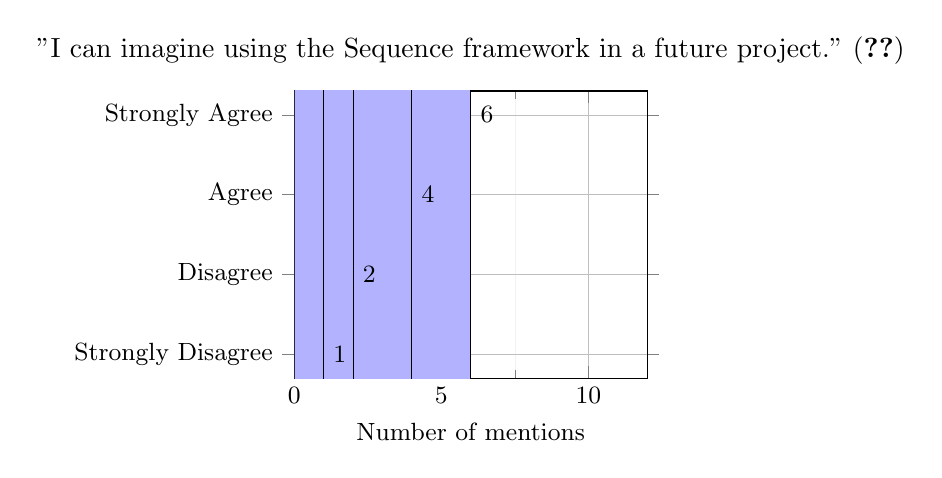
\begin{tikzpicture}
\begin{axis}[
% instead of scaling
width=\textwidth / 2, % Breite des Charts
title={"I can imagine using the Sequence framework in a future project."~(\ref{sub:ut_q4})},
xbar,  % Art des Charts                                            
xmin=0, % y min
xmax=12, % y max
%ylabel style={color=darkgray},
ticklabel style={font=\small},
label style={font=\small},
nodes near coords style={font=\small},
bar width=20, % Breite der Balken (in points)
nodes near coords, % Labels oberhalb der Bars
xlabel={Number of mentions},
grid=both, % Zeilen ds Grids
grid style={line width=.1pt, draw=gray!10},
major grid style={line width=.2pt,draw=gray!50},
minor x tick num=1,
ytick=data,
% use explicit ticklabels instead of symbolc x coords
yticklabels={Strongly Agree, Agree, Disagree, Strongly Disagree},
]
\addplot[black,fill=blue!30!white]
coordinates{ (6,4) (4,3) (2,2) (1,1) };
\end{axis}
\end{tikzpicture}
\caption{Responses to "I can imagine using the Sequence framework in a future project."}
\label{fig:usertest_q1}
\end{figure}
% subsubsection Conclusion (end)
% subsection Findings Sequence library(end)
\subsection{Findings for JINQ} % (fold)
\label{sub:Findings for JINQ}
\subsubsection{Findings and Improvements} % (fold)
\label{subsub:jinq_finding_and_imrpovements}

We decided to include following findings into JINQ:
\begin{itemize}
  \item \textbf{Better Introduction to JINQ}: Two people suggest using
    |JSONMonad()| directly inside of |from| (text answer~\ref{sub:ut_q13}).
    However, this makes no sense since JINQ can handle arbitrary monads. Thus,
    the documentation provided did not provide a sufficient overview.
    Therefore, the JSDoc of JINQ must give a better introduction to the topic.
    Additional examples should show the usage using different monads.
  \item \textbf{Revise JSDoc (functions and examples)}: Nearly a quarter of the participants found JINQ
    challenging (\ref{sub:ut_q8}). This shows that these concepts needed to be
    sufficiently well introduced. From the solutions given to us, it is evident
    that more JSDoc was required. In addition, more examples would coin to a
    better understanding (text answer~\ref{sub:ut_q13}).
    \item \textbf{Not exactly the same as SQL}: Two people needed help with
      JINQ not writing exactly like SQL (handed in code). An SQL query
      |Select NAME from PERSON where AGE > 18| is translated into JINQ via
      |from(PERSON).where(p => p.age > 18).select(p => p.name);| So the order
      of |select| and |where| is reversed. So the JSDoc of JINQ needs to
      mention more clearly that working with JINQ is different than working
      with SQL.
\end{itemize}

The following are great ideas but are beyond the scope of this project to
implement. Find detailed information about all of them in the
Section~\ref{sub:JINQ Functions}.
\begin{itemize}
  \item \textbf{Error handling}: Several people had trouble with null values,
    mainly when, for example, when calling a  function on a non-existent object
    property in a |select| or a |where| (text answer~\ref{sub:ut_q13}, and
    handed in solution). In the discussion, the idea came up to
    provide functions like |notNull|, |safeWhere| or |safeMap| to catch this.
\end{itemize}
% subsubsection Findings and Improvements (end)
\subsubsection{Conclusion} % (fold)
\label{subsub:Conclusion}
Although JINQ still has room for improvement, the general feedback is very
good. Almost all find it helpful to search JSON structures using JINQ
(\ref{sub:ut_q10}). The majority already found the current state of JINQ easy
to use \ref{sub:ut_q8}.

As Figure~\ref{fig:usertest_q2} shows, most people think that JINQ can be an asset in a future
project:
\begin{figure}[H]
\centering
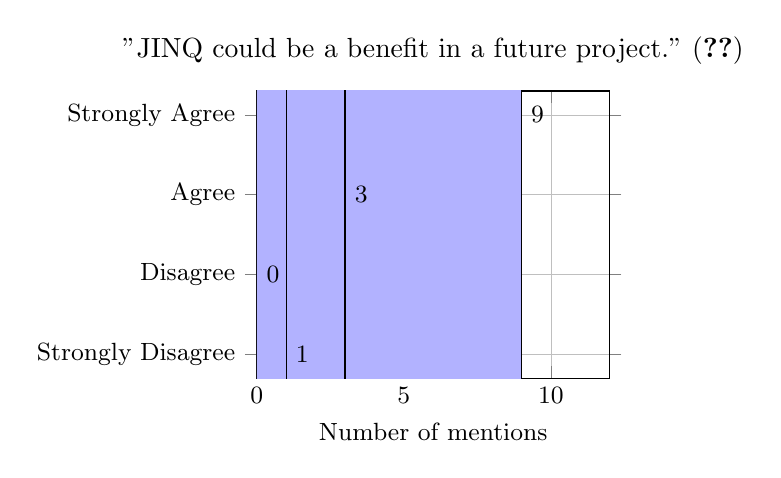
\begin{tikzpicture}
\begin{axis}[
% instead of scaling
width=\textwidth / 2, % Breite des Charts
title={"JINQ could be a benefit in a future project."~(\ref{sub:ut_q12})},
xbar,  % Art des Charts                                            
xmin=0, % y min
xmax=12, % y max
%ylabel style={color=darkgray},
ticklabel style={font=\small},
label style={font=\small},
nodes near coords style={font=\small},
bar width=20, % Breite der Balken (in points)
nodes near coords, % Labels oberhalb der Bars
xlabel={Number of mentions},
grid=both, % Zeilen ds Grids
grid style={line width=.1pt, draw=gray!10},
major grid style={line width=.2pt,draw=gray!50},
minor x tick num=1,
ytick=data,
% use explicit ticklabels instead of symbolc x coords
yticklabels={Strongly Agree, Agree, Disagree, Strongly Disagree},
]
\addplot[black,fill=blue!30!white]
coordinates{(9,4) (3,3) (0,2) (1,1)};
\end{axis}
\end{tikzpicture}
\caption{Responses to "JINQ could be a benefit in a future project."}
\label{fig:usertest_q2}
\end{figure}
% subsubsection Conclusion (end)
% subsection Findings for JINQ (end)
\subsection{General Findings} % (fold)
\label{sub:General Findings}
The questionnaire concludes with general questions. Among other things, the
closing explains how effectively IDEs support JSDoc and whether the testers
find this useful. Most participants used IntelliJ or WebStorm for testing
(~\ref{sub:ut_q15}). Figure~\ref{fig:usertest_q3} shows that the IDE was an excellent help for this test. Thus, It
makes sense to write a detailed JSDoc. Code navigation, code completion, etc.,
are also popular with users in JavaScript. With the right IDEs, this also works
very well.
%\begin{figure}[H]
%\begin{tikzpicture}
%\begin{axis}[
%% instead of scaling
%width=\textwidth / 2, % Breite des Charts
%title={"My IDE provided me with helpful support during the user test." (\ref{sub:ut_q16})},
%ybar,  % Art des Charts                                            
%ymin=0, % y min
%ymax=12, % y max
%%ylabel style={color=darkgray},
%%xlabel style={font=\small},
%bar width=20, % Breite der Balken (in points)
%nodes near coords, % Labels oberhalb der Bars
%ylabel={Number of mentions},
%grid=both, % Zeilen ds Grids
%grid style={line width=.1pt, draw=gray!10},
%major grid style={line width=.2pt,draw=gray!50},
%minor y tick num=4,
%xtick=data,
%% use explicit ticklabels instead of symbolc x coords
%xticklabels={Strongly Agree, Agree, Disagree, Strongly Disagree},
%xticklabel style={ rotate=-20 },
%]
%\addplot[black,fill=blue!30!white]
%coordinates{ (1,10) (2,2) (3,1) (4,0) };
%\end{axis}
%\end{tikzpicture}

\begin{figure}[H]
\centering
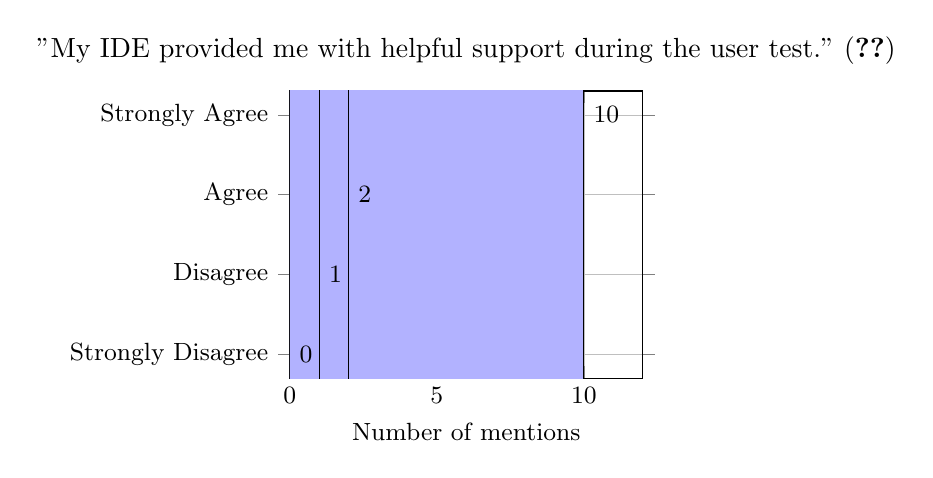
\begin{tikzpicture}
\begin{axis}[
% instead of scaling
width=\textwidth / 2, % Breite des Charts
title={"My IDE provided me with helpful support during the user test." (\ref{sub:ut_q16})},
xbar,  % Art des Charts                                            
xmin=0, % y min
xmax=12, % y max
%ylabel style={color=darkgray},
ticklabel style={font=\small},
label style={font=\small},
nodes near coords style={font=\small},
bar width=20, % Breite der Balken (in points)
nodes near coords, % Labels oberhalb der Bars
xlabel={Number of mentions},
grid=both, % Zeilen ds Grids
grid style={line width=.1pt, draw=gray!10},
major grid style={line width=.2pt,draw=gray!50},
minor x tick num=1,
ytick=data,
% use explicit ticklabels instead of symbolc x coords
yticklabels={Strongly Agree, Agree, Disagree, Strongly Disagree},
]
\addplot[black,fill=blue!30!white]
coordinates{ (10,4) (2,3) (1,2) (0,1) };
\end{axis}
\end{tikzpicture}
\caption{Responses to "My IDE provided me with helpful support during the user
test."}
\label{fig:usertest_q3}
\end{figure}

% subsection General Findings (end)
\subsection{Conclusion} % (fold)
\label{sub:Conclusion}

This user test shows that the features this library brings are beneficial. In
addition, it offers some improvement points of the API. Implementing the
documented hints improves the quality and usability of this library even more.
We are delighted with the result. Of course, we are especially pleased with the
text responses - many further underline the positive attitude towards this
library. 

% subsection Conclusion (end)
% section User Test Evaluation (end)

\section{Examples} % (fold)
\label{sec:Examples}
This section shows some examples implemented with the
Sequence library to demonstrate its variable usage.
The following covers easy-to-understand and more sophisticated
examples. Consult the listed sources to understand the applications
thoroughly if something is unclear.

\subsection{Fibonacci Sequence}
\label{sub:Fibonacci Sequence}
This is an example of a specialized sequence constructor.
Listing~\ref{lst:fibonacci_sequence} shows the implementation of the Fibonacci 
sequence~\cite[p.~36]{math_diskrete_2011}:
\begin{lstlisting}[
  style=ES6, 
  caption=FibonacciSequence implementation,
  label={lst:fibonacci_sequence}
  ]
const start   = Pair(0)(1);
const whileFn =  _ => true;
const incrFn  = ([fst, snd]) => Pair(snd)(fst + snd);
/**
 * Generates the Fibonacci sequence.
 *
 * @constructor
 * @pure
 * @returns { SequenceType<Number> }
 *
 * @example
 * const result = take(8)(FibonacciSequence);
 *
 * console.log(...result);
 * // => Logs '1, 1, 2, 3, 5, 8, 13, 21'
 */
const FibonacciSequence = 
                    map(pair => pair(snd))(Sequence(start, whileFn, incrFn));
\end{lstlisting}
The |FibonacciSequence| constructor generates the Fibonacci sequence using the
|Sequence| and |Pair| constructors. The incrementation function produces a pair
containing the last returned value and the value to be returned.  The |map|
function then extracts the current Fibonacci number from the pair returned by
the sequence.

\subsection{Fizz Buzz}
\label{sub:Fizz Buzz}
Fizz Buzz is a simple game played with numbers, typically in a group setting. Players
take turns counting upward, but instead of saying numbers divisible by 3, they
say "Fizz", and instead of numbers divisible by 5, they say "Buzz". If a number
is divisible by both 3 and 5, they say "FizzBuzz". This game also serves as a 
programming task.
\newline
Frege Goodness~\cite{frege_goodness} includes a detailed explanation of the
game. 

First, let us look at the game's simplest form in listing~\ref{lst:simple_fizzbuzz}. 
The fizzes and buzzes are combined in a sequence. 
The sequence returns a number if neither a fizz nor a buzz occurs:

\begin{lstlisting}[
  style=ES6, 
  caption=Fizz Buzz example,
  label={lst:simple_fizzbuzz}
  ]
const limit    = 15;
const range    = Range(1, limit);
const fizzez   = cycle(["", "", "fizz"]);
const buzzez   = cycle(["", "", "", "", "buzz"]);

const pattern  = zipWith((fizz, buzz) => fizz + buzz)(fizzez)(buzzez);
const fizzbuzz = zipWith((num, str) => str === "" ? num : str)(range)(pattern);

console.log(...take(limit)(fizzbuzz));
// => Logs '1 2 "fizz" 4 "buzz" ... 11 "fizz" 13 14 "fizzbuzz"'
\end{lstlisting}

As you observe, the entire setup relies on sequences. We define three
distinct endless sequences. A range generates a line of numbers, while |cycle|
produces an unending repetition for "fizzes" and "buzzes". Memory usage remains
minimal. Subsequently, |zipWith| merges the individual sequences and yields a
new sequence. This uncomplicated setup underscores that working with sequences
is declarative, straightforward and highly understandable.

Now we are extending the application to add new rules during the runtime:

\begin{lstlisting}[
  style=ES6, 
  caption=Fizz Buzz example extended,
  label={lst:fizz_buzz}
  ]
import * as _ from "./src/sequence/sequence.js";

const infiniteNumbers = _.Sequence(1, _ => true, i => i + 1);

const createSequenceForRule = rule =>
  _.pipe(
    // add rule's text to number
    _.map(a => a === rule.getNr() ? rule.getText() : ""),     
    _.take(rule.getNr()), // abort on this rules number
    _.cycle
  )(infiniteNumbers);

const buildFizzBuzz = () => {
  const currentRules = model.rulesSnapshot().map(createSequenceForRule);
  const baseLine     = _.Sequence("", _ => true, _ => "");

  const fizzBuzz = _.pipe(
      // reduce to single sequence by combining all iterable values
    _.reduce$((acc, cur) => _.zipWith((a, b) => a + b)(acc)(cur), baseLine), 
    _.zipWith((numbers, pattern) => pattern === "" ? String(numbers) : pattern)
                 (infiniteNumbers), 
    // limit output
    _.take(model.getUpperBoundary()),
    _.drop(model.getLowerBoundary() -1),
  )(currentRules);

  model.setResult(fizzBuzz);
};
\end{lstlisting}
Listing~\ref{lst:fizz_buzz} shows two functions, |createSequenceForRule|, and
|buildFizzBuzz|. \\ 
|createSequenceForRule| is called with an argument |rule| representing a
number and a string. The returned infinite sequence then contains the
corresponding text at each multiple of the rules number. In the remaining
places, it contains an empty string. \\ 
Calling |createSequenceForRule(Rule(3, "fizz"))| thus creates a sequence
generating |"", "", "fizz", "", "", "fizz", ...|.\\
The function |buildFizzBuzz| reduces all sequences representing a rule to a
single sequence. 
Figures~\ref{fig:fizzbuzz_control} and \ref{fig:fizzbuzz_result} demonstrate a
screenshot of a simple application showing two rules and the resulting sequence.
The implementation enables adding new rules at runtime.

\begin{figure}[H] \centering \begin{minipage}{.5\textwidth} \centering
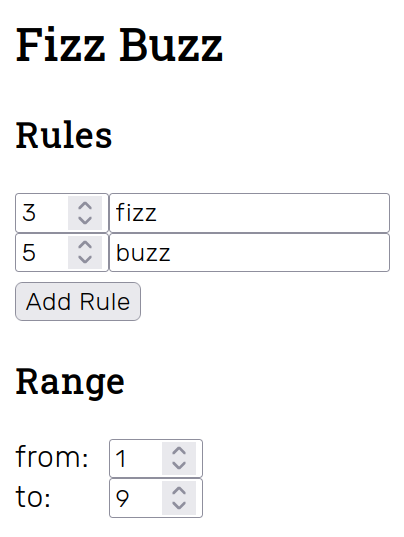
\includegraphics[width=.6\linewidth]{./mainmatter/pictures/fizzbuzz_control.png}
\captionof{figure}{Fizz Buzz controls} \label{fig:fizzbuzz_control}
\end{minipage}%
\begin{minipage}{.5\textwidth}
  \centering
  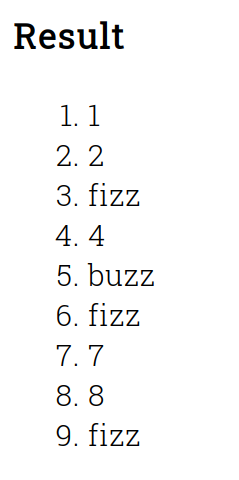
\includegraphics[width=.4\linewidth]{./mainmatter/pictures/fizzbuzz_result.png}
  \captionof{figure}{Fizz Buzz result}
  \label{fig:fizzbuzz_result}
\end{minipage}
\end{figure}

\subsection{JINQ}
\label{sub:results JINQ}
The following examples use |JINQ| to browse and process JSON files.

\subsubsection{Find all Students}
\label{subsub:Find all Students}
We want to filter out all participants that have a student ID. As you can see
in the excerpt of the JSON file in listing~\ref{lst:json_file_devs}, the
property |switch-edu-id| is not defined for all people. Because the
|JsonMonad| works in the background with a maybe, such situations can be
processed without null handling.

\begin{lstlisting}[
  style=json, 
  caption=Excerpt of a JSON File including developers,
  label={lst:json_file_devs}
  ]
[
  {
    "id": 1,
    "name": "",
    "age": 28,
    "salary": 50000,
    "favoriteLanguages": [1, 3, 5]
  },
  {
    "id": 2,
    "switch-edu-id": "12-432-23",
    "name": "Emma Johnson",
    "age": null,
    "salary": 60000,
    "favoriteLanguages": [2, 4]
  },
  {
    "id": 3,
    "name": "Sophia Davis",
    "age": 40,
    "salary": null,
    "favoriteLanguages": [null, 4, 5]
  },
  ...
 ]
\end{lstlisting}

Using JINQ it is straightforward to access the desired students by just using
the function |where|:

\begin{lstlisting}[
  style=ES6, 
  caption=JINQ Example - find all students,
  label={lst:jinq_find_students}
  ]
const findAllStudentIds = developers => {
  const allIds =
    from(JsonMonad(developers))
      .select(x => x['switch-edu-id'])
      .result();
};
\end{lstlisting}

\subsubsection{Find Sophia's Programming Languages}
\label{subsub:Find Sophia's Programming Languages}

This example combines two JSON files. We use the JSON file from the previous
example and the one from listing~\ref{lst:json_file_lang} below.
Listing~\ref{lst:jinq_sophias_langs} shows the code that finds Sophia's 
favourite programming languages by combining two JSON files using |pairWith|. 

\begin{lstlisting}[
  style=json, 
  caption=Excerpt of a JSON File including programming languages,
  label={lst:json_file_lang}
  ]
[
  {
    "id": 1,
    "name": "Java"
  },
  ...
  {
    "id": 4,
    "name": "C++"
  },
  {
    "id": 5,
    "name": "Haskell"
  }
]
\end{lstlisting}
This is also comparatively easy to do with JINQ. |pairWith| allows adding a
second data source to the current one, forming all possible combinations. The
function |where| then keeps only the needed pairs. A simple mapping at the end
outputs the names of the programming languages.
\begin{lstlisting}[
  style=ES6, 
  caption=JINQ example - find Sophia's programming languages,
  label={lst:jinq_sophias_langs}
  ]
const sophiasProgrammingLanguages = (devs, languages) =>
    from(JsonMonad(devs))
      .where   ( dev    => dev.name === "Sophia Davis")
      .select  ( sophia => sophia.favoriteLanguages)
      .pairWith( JsonMonad(languages) )
      .where   ( ([langId, language]) => langId === language.id )
      .select  ( ([     _, language]) => language.name )
      .result  ();
\end{lstlisting}

\subsection{Numerical Differentiation}
\label{sub:Numerical Differentiation}
This example shows a mathematical use case, the numerical differentiation using
sequences:

\begin{lstlisting}[
  style=ES6, 
  caption=Differentiation using sequences,
  label={lst:diff_sequences}
  ]
const halve   = x => x / 2;
const repeatF = (f, x) => _.Sequence(x, _ => true, f);
const halves = h0 => repeatF( halve, h0);

const slope = f => x => h => (f(x + h) - f(x)) / h;
const differentiate = h0 => f => x => _.map ( slope(f)(x) ) (halves(h0));
\end{lstlisting}

Listing~\ref{lst:diff_sequences} implements the following steps: 


\begin{itemize}
  \item{|repeatF| repeatedly applies the function $f$ to a value of the
    previous calculated result, starting with $x$.}
  \item{ |halves| is using |repeatF| and |halve| to halve a value $h0$.} 
    \item{|slope| calculates the slope of a function $f$ at the position $x$
      with delta $h$.}
 \end{itemize}

This code already provides everything needed for differentiation. The function
|differentiate| calculates the slope of a function at a given point $x$ more
and more exactly.
Listing~\ref{lst:diff_seq_parabola} uses these functions to determine the 
slope at $x = 1$ of the function |parabola| defined on line~\ref{line:diffs}:

\begin{lstlisting}[
  style=ES6, 
  caption=Differentiation using sequences,
  label={lst:diff_seq_parabola}
  ]
const parabola = x => x * x; *'\label{line:diffs}'*

const diffs = differentiate(0.5)(parabola)(1);
\end{lstlisting}

Since |diffs| contains an infinite sequence, one further
function is still needed.
Listing~\ref{lst:impl_within} shows the function |within|, which allows
differentiating until two successive values are smaller than a given epsilon:

\begin{lstlisting}[
  style=ES6, 
  caption=Implementation of within,
  label={lst:impl_within}
  ]
const within = eps => sequence => {
  const [a, rest] = _.uncons(sequence);
  const [b]       = _.uncons(rest);
  const diff      = Math.abs(a - b);

  if (diff <= eps) return b;
  return within(eps)(rest);
};
const slopeOfFAtX = within(0.000_1)(diffs);
\end{lstlisting}

Listing~\ref{lst:impl_within} defines the following implementations:

\begin{itemize}
  \item |within| calculates recursively the slope of the |parabola| using the
    sequence |diffs| until a satisfying accuracy. Because of the laziness of
    the sequence, |within| only calculates as many slopes as needed!
  \item At the end, |slopeOfFAtX| calculates the slope with the given parameters.
\end{itemize}


\subsection{Tic Tac Toe with a Kind of AI}
\label{sub:Alpha - Beta Algorithm}
This section describes the implementation of the alpha-beta heuristic in
JavaScript, an algorithm for estimating how good a position a game player is
in. \\ 
This algorithm allows for building a computer-controlled opponent for a
turn-based game. Hughes explains how the algorithm uses laziness and
higher-order functions to be modular and extensible in his paper.~\cite[p.
16]{hughes_why_1989}. As chapter~\ref{chap:Modularizing Programs} describes, the
Sequence library supports these two concepts, thus allowing to port the
algorithm to JavaScript.

\subsubsection{How does the Algorithm work?} % (fold)
\label{subsub:How does the Algorithm work?}
The following explanation is meant to give a brief overview for the
algorithm, allowing to understand the preceding code. For a deeper
understanding of the algorithm, consider ~\cite[Ch. 5]{hughes_why_1989} or the
section "Incremental Development" in Frege Goodness~\cite{frege_goodness}.

\paragraph{Building a Game Tree} The idea of the algorithm is to build a tree
containing \textit{all} possible playing fields. The start node in this
tree is the current state of the playing field. Its children are all possible
playing fields, which can arise when the players make their next moves. This
results in a potentially endless tree. All direct successors of a node are the
next possible moves for this node's playing field. Since this tree can be huge,
depending on the game, even infinitely large, only a lazy data structure can
handle it!\\
The algorithm must estimate whether a playfield is good or bad for a player to
find the best possible next move. The simplest way to figure this out is to
look at the playing field and decide if a player has already won. In the case
of tic tac toe, a player has won when three of his symbols are next to each
other. \\
A function (called |evalFunction|) does this evaluation - if the algorithm has
won the game on a field, it evaluates to 1 if it has lost to -1, in all other
cases, to 0.\\
The |evalFunction| is mapped over the tree (where higher-order functions come
into play) - each node is assigned its static value, saying how promising the
playfield of this node is. This results in a new tree with the value of
|evalFunction| assigned to the nodes instead of all possible fields.\\

\paragraph{What is the best Move?}
The tree's root is the current playing field - the algorithm cannot know from
the root which moves are good and which are not. The previously mentioned
|evalFunction| will evaluate to 0 for most nodes directly after the root.
Therefore, the computer also calculates subsequent moves. The values of the
lowest calculated nodes are then propagated upwards to the root. 

The function |maximize| goes through to the lowest precalculated level. It
evaluates the board there: when it is the computer's turn, it selects the board with
the highest value assigned (safest chance of winning). If it is the opponent's
turn, it selects the smallest value (the algorithm thus assumes that the
opponent also selects the best possible move). This found value is assigned to
the parent node as a result - and chooses the best move on this level according
to the same scheme. Ultimately, the root has the value with the best possible
chances of winning!

\paragraph{How to evaluate the huge Tree?} The tree of possible moves and possible
result values can be huge. So the algorithm must have a way to limit the tree
to a fixed depth. The algorithm uses pruning - from a freely selectable depth,
it cuts the children off. 

\subsubsection{Implementation}
\label{subsub:alphabeta_implementation}
\paragraph{Basic Types and Helper functions} 
Listing~\ref{lst:tictactoe_types} shows the required types for the game
implementation. \\
A pair models the |Tree| (line~\ref{line:ttt_treetype}) - the first
value is the current node, and the second value is a sequence consisting of
further trees. The types |Player| and |Stone| exist only for writing more
expressive JSDoc.

\begin{lstlisting}[
  style=ES6, 
  caption=Tic tac toe types,
  label={lst:tictactoe_types}
  ]
/**
 * 
 * @template _T_
 * @typedef {SequenceType<Tree<_T_>>} TreeSequence
 */

/** *'\label{line:ttt_treetype}'*
 * @template _T_
 * @typedef { PairSelectorType<_T_, TreeSequence<_T_>> } Tree
 */


/**
 * @typedef { "Computer" | "Human" | "NoPlayer" } Player
 */

/**
 * @typedef { 1 | -1 | 0 } Stone
 */

/**
 * @typedef Board
 * @property { Player } whosTurn
 * @property { Iterable<Stone>} fields - A board has fields from 0 to 8.
 */
\end{lstlisting}

Listing~\ref{lst:tictactoe_players} includes the definition of the players and some
functions used in the game process. Since JavaScript does not support pattern
matching, the functions |opponent| and |stone| use a workaround - they store
the mappings in an object.

\begin{lstlisting}[
  style=ES6, 
  caption=The players and some helper functions,
  label={lst:tictactoe_players}
  ]
/** @type { Player } */
const Computer = "Computer";

/** @type { Player } */
const Human = "Human";

/** @type { Player } */
const NoPlayer = "NoPlayer";

/**
 * Returns the opponent of a given player.
 * @param { Player } player
 * @return Player
 */
const opponent = player => {
  const pairings = {
    "Computer" : Human,
    "Human"    : Computer,
    "NoPlayer" : NoPlayer,
  };
  return pairings[player];
};

/**
 * Returns the stone number of a given player.
 * @param { Player } player
 * @returns Stone
 */
const stone = player => {
  const pairings = {
    "Computer" :  1,
    "Human"    : -1,
    "NoPlayer" :  0,
  };
 return pairings[player];
};

/**
 * Transforms each board element using the given function f.
 * @template _T_, _U_
 * @type {
 *         (f: (Board) => _T_)
 *      => (tree: Tree<_U_>)
 *      => Tree<_T_>
 * }
 */
const treeMap = f => ([a, sub]) => Pair(f(a))(map(treeMap(f))(sub));
\end{lstlisting}

\paragraph{Building trees and processing the Game Board} 
Listing~\ref{lst:tictactoe_gametree} shows the functions for building a game
tree. |unfold| is a function that takes a value (for example, a board) and
creates new values of the same types of it (for example, all boards possibly
arising in one move).
\begin{lstlisting}[
  style=ES6, 
  caption=Tic tac toe game tree,
  label={lst:tictactoe_gametree}
  ]
/**
 * Generates recursively a game tree, which is potentially endless.
 * @template _T_
 * @type {
 *       (unfold: ((_T_) => Iterable<_T_>))
 *    => (a: _T_)
 *    => Tree<_T_>
 * }
 */
const buildTree = unfold => a => {
  const as = unfold(a);
  const children = map(buildTree(unfold))(as);
  return Pair(a)(children);
};

/**
 * Creates a game tree.
 * @param { Board } board
 * @returns Tree<Board>
 */
const gameTree = board => buildTree(moves)(board);
\end{lstlisting}

Listing~\ref{lst:tictactoe_move} includes the |moves| function. This function
calculates all possible moves for a player based on the current playing field.
If a player has already won, it returns an empty sequence.
\begin{lstlisting}[
  style=ES6, 
  caption=Tic tac toe move function,
  label={lst:tictactoe_move}
  ]
/**
 * Indexes each field using a {@link PairType}.
 * @param { Iterable<Stone> } fields
 * @return { SequenceType<PairType<Stone, Number>> }
 */
const indexFields = fields => zip(fields)(Range(1,9));

/**
 * Calculates possible moves for a given board.
 * @param { Board } board
 * @return SequenceType<Board>
 */
const moves = board => {
  if (hasWon(board)(Computer)) return /**@type {SequenceType<Board>} */nil;
  if (hasWon(board)(Human))    return /**@type {SequenceType<Board>} */nil;

  const otherPlayer   = opponent(board.whosTurn);
  const indexedFields = indexFields(board.fields);

  const blankIndices =
    from(indexedFields)
      .where( ([content, _]) => content === stone(NoPlayer))
      .select( ([_, i]) => i)
      .result();

  const fieldsWithPlayerPlacedAt = pos =>
    from(indexedFields)
      .select(([content, i]) => i === pos ? stone(board.whosTurn) : content)
      .result();

  const boardFieldsAfterMove = map (fieldsWithPlayerPlacedAt) (blankIndices);

  return map(fields => ({fields, whosTurn: otherPlayer})) (boardFieldsAfterMove);
};
\end{lstlisting}

\paragraph{Evaluating a Board}
Listing~\ref{lst:tictactoe_hasWon} shows the implementation of the |hasWon|
function, which checks if a player has won on a given board. The evaluation
function, explained in section ~\ref{subsub:How does the Algorithm work?}, uses
this function to assess a playing field. Line~\ref{line:ttt_static_eval}
defines this function called |staticEval|.

\begin{lstlisting}[
  style=ES6, 
  caption=Tic tac toe hasWon function,
  label={lst:tictactoe_hasWon}
  ]
/**
 * Checks, if a player has won.
 * @type {
 *    (board: Board)
 *    => (player: Player)
 *    => Boolean
 * }
 */
const hasWon = board => player => {
  const winTriples = [
    [1,2,3], [4,5,6], [7,8,9], // row
    [1,4,7], [2,5,8], [3,6,9], // col
    [1,5,9], [3,5,7]           // diag
  ];

  const checkTriple = triple => {
    const actualStone   = stone(player);
    const indexedFields = indexFields(board.fields);

    const playerOnFields =
      from(indexedFields)
      .where( ([_, i])        => triple.includes(i))
      .select( ([content, _]) => content === actualStone)
      .result();

    return foldl$((acc, cur) => acc && cur, true)(playerOnFields);
  };
  return pipe(
    map(checkTriple),
    foldl$((acc, cur) => acc || cur, false)
  )(winTriples)
};

/**
 * Evaluates a given board.
 * @param { Board } board
 * @returns Number
 */
const staticEval = board => {*'\label{line:ttt_static_eval}'*
  if (hasWon (board) (Computer)) return 1.0;
  if (hasWon (board) (Human))    return -1.0;
  return 0.0;
};

\end{lstlisting}

\paragraph{Finding the best Move}
Listing~\ref{lst:tictactoe_minimax} shows the implementation of the functions
|maximize| (and its counterpart |minimize|) explained in
section~\ref{subsub:How does the Algorithm work?}. These functions determine
which are the best moves.

\begin{lstlisting}[
  style=ES6, 
  caption=Tic tac toe minimax algorithmus,
  label={lst:tictactoe_minimax}
  ]
/**
 * Determines the best move.
 * @template _T_
 * @param { Tree<_T_>}
 * @return { _T_ }
 */
const maximize = ([a, sub]) => {
  if (sub ["=="] (nil)) return a;
  return max$ (map(minimize)(sub))
};

/**
 * Determines the best move for the opponent.
 * @template _T_
 * @param { Tree<_T_>}
 * @return { _T_ }
 */
const minimize = ([a, sub]) => {
  if (sub ["=="] (nil)) return a;
  return min$ (map(maximize)(sub))
};
\end{lstlisting}

\paragraph{Pruning Trees} 
We cut off (prune) the possibly infinite tree. The following
listing~\ref{lst:tictactoe_prune} shows the implementation of this pruning.
Since subtrees are sequences, |nil| replaces them when pruning.

\begin{lstlisting}[
  style=ES6, 
  caption=Tic tac toe prune function,
  label={lst:tictactoe_prune}
  ]
/**
 * Prunes a given {@link Tree} to a max depth n.
 * @template _T_
 * @type {
 *           (n: Number)
 *        => (tree: Tree<_T_>)
 *        => Tree<_T_>
 * }
 * @param n
 */
const prune = n => tree => {
  const [a, sub] = tree;
  if (n === 0) return Pair(a)(nil);
  else return Pair(a)(map(prune(n-1))(sub));
};
\end{lstlisting}

\paragraph{Putting it all together}
The following functions evaluate a playing field. \\ 
The function |nextBoard| calculates the best possible next move for the
computer. The number |lookaheads| defines how many turns the algorithm
calculates in advance. Based on these calculations the algorithm chooses the
next move.

\begin{lstlisting}[
  style=ES6, 
  caption=Tic tac toe - evaluating functions,
  label={lst:tictactoe_eval}
  ]
/**
 * Evaluates a given Board by building a tree
 * @type {
 *            (lookahead: Number)
 *         => (board: Board)
 *         => Number
 * }
 */
const evaluate = lookahead => board => {
  const prunedTree = prune(lookahead)(gameTree(board));
  const mappedTree = treeMap(staticEval)(prunedTree);
  return minimize(mappedTree);
};

/**
 * @template _T_
 * @type {
 *            (lookahead: Number)
 *         => (board: Board)
 *         => PairSelectorType<_T_, Board>
 * }
 */
const nowValue = lookahead => board =>
  Pair(evaluate(lookahead)(board))(board);

/**
 * Calculates the next board with given board fields.
 * @type {
 *          (lookahead: Number)
 *       => (inFields: Array<Number>)
 *       => Board
 * }
 */
const nextBoard = lookahead => inFields => {
  const currentBoard = { whosTurn: Computer, fields: inFields };
  // get all possible
  const possibleMoves  = moves (currentBoard);
  if (isEmpty(possibleMoves)) return currentBoard;
  // evaluate each move by looking ahead how good it is
  let evaluatedMoves =  map (nowValue(lookahead)) (possibleMoves);

  // if the computer is sure to lose 
  // only look one place ahead to prevent the "nearest" loss
  if (onlyLoses(evaluatedMoves)) {
    evaluatedMoves = map (nowValue(1)) (possibleMoves);
  }

  /**
   * Gets the highest ranked board of the passed board
   * @param {SequenceType<PairSelectorType<Number, Board>>} boards
   * @return Board
   */
  return bestOf(evaluatedMoves);
};
\end{lstlisting}

\subsubsection{The Result} % (fold)
\label{sec:ttt_result}
One advantage of JavaScript is that it works hand in hand with websites and
HTML. A website with a UI (like figure~\ref{img:ttt_playfield}) can now use the
algorithm:\\

\begin{figure}[H]
    \centering
    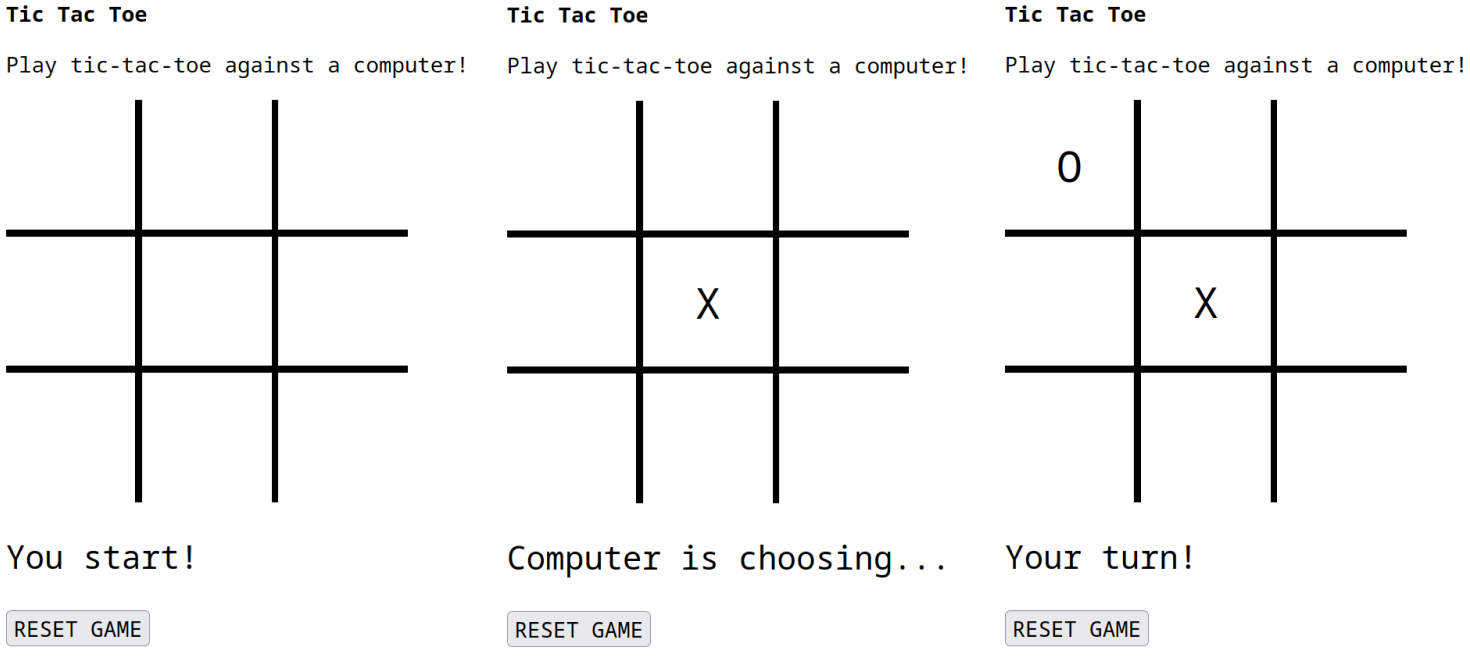
\includegraphics[width=0.9\textwidth]{./mainmatter/pictures/tic-tac-toe-field.png}
    \caption{A website using the algorithm}
    \label{img:ttt_playfield}
\end{figure}

When a player places his stone on the board, the function |nextBoard| gets
called. The algorithm automatically makes the best possible next turn based on
how many moves it can look ahead and returns the new board.
% subsubsection The result (end)

\subsubsection{Conclusion} % (fold)
\label{subsub:ttt_conclusion}
This example shows impressively how the Sequence library enables developers to
adapt an algorithm developed for functional programming languages in
JavaScript.\\
Of course, copying the algorithm is impossible because JavaScript misses some
language features like pattern matching. Nevertheless, the essential concepts
and logic of the algorithm can be adopted directly! \\
It is also exciting how JSDoc allows constructing straightforward talking types
like |Player| or |Stone| (listing~\ref{lst:tictactoe_types}).\\
To extend the algorithm, for example, to improve the static evaluation to
decide how good a current playing field is, only one function has to be
adjusted. Also, the evaluation of the algorithm can be easily improved and
detached from other logic by increasing the number of lookahead moves. Further
optimizations to prune away subtrees that are out of consideration anyway can
be done directly in the function |maximize|.\\
Thus, the modularity and extensibility of the program is very high.
% subsubsection Conclusion (end)

\section{Future Features}
\label{sec:Future Features}
This chapter covers unimplemented functions. These include implementations that
were no longer possible during the work or resulted from user testing feedback.
The following articles describe the most relevant features and explain why it
makes sense to implement them at a future point in time.

\subsection{Logging}
\label{sub:Logging}
Logging is a topic that has come up several times. It appears, on one hand,
during the implementation of the Sequence Library, but also through as feedback
from a test proband. In our computer science project work from the fifth
semester IP5 we had to implement a logging framework. This would also be useful
to include in the Sequence Library. Especially in case of errors, analyzing
messages from the involved functions would be helpful. Currently, the logging
framework is only included in a part of the test framework. But this could be
extended in a next step.

\subsection{Operators and Operations}
\label{sub:Operators and Operations}

\subsubsection{uncons}
\label{subsub:uncons}
|uncons| is an operation that returns the first and the rest of an iterable in a
pair. Basically, this operation is already included in the sequence library.
But only as an un-safe variant. That means, |uncons| applied to an empty list
fails. Thus one would have a version, which for example, wraps the result in a
|MaybeType|. |uncons| on an empty list would then return |Nothing|. The
api documentation page~\cite{hoogle_uncons} describes the function in detail.

\subsubsection{tail}
\label{subsub:tail}
|tail| ~\cite{hoogle_tail} is a useful function that removes the first element of an |Iterable|
and returns the rest of it. By implementing tail, one have to pay attention to
empty |Iterable| single element case. An option could be to return a
|MaybeType|. |Nothing|, if the list has one or zero elements, and
|Just| including the result otherwise.

\subsubsection{unfoldr}
\label{subsub:unfoldr}
|unfoldr| is a powerful concept of creating sequences of data. It would
supplement the options to make new |Iterable| beside the |Sequence|
constructor. It works on a |MaybeType|. |unfoldr| creates an |Iterable| which returns
a |PairType| wrapped in Just with the value of the current iteration and the next
element. If the stop condition is fulfilled, |unfoldr| return |Nothing|. For
further information, have a look at the documentation on hoogle~\cite{hoogle_unfoldr}.

\subsubsection{iterate}
\label{subsub:iterate}
|iterate| takes two arguments. The first argument is a function, and the second
is a start value. It generates an infinite |Iterable| of repeated applications of
the function to the calculated value. You will find more information about
|iterate| on hoogle~\cite{hoogle_iterate}.

\subsection{JINQ Functions}
\label{sub:JINQ Functions}
It is possible to get errors when working with JINQ and JSON Monad by grabbing
not present values. That means if a function in select accesses a property
which is not defined, it will throw an error. This kind of null-case handling
takes a lot of work. To remedy this situation, having error-safe functions like
|safeSelect| to access probably present values would be excellent.

\subsection{Applications}
\label{sub:Applications}
\subsubsection{Fixpoint Sequence}
\label{subsub:Fixpoint Sequence}
In the mathematical context, having a tool for approximations is helpful. A
constructor for such a case could be the Fixpoint Sequence. It allows us to
find an approximation with a given number of iterations or by providing a value
of minimal deviation.

\subsubsection{A Kind of Scalpel}
\label{subsub:A Kind of Scalpel}
Scalpel~\cite{scalpel} is a Haskell library to scrap web content. Building a similar
application based on the present implementations could be possible. With JINQ
and |JsonMonad|, we already have a scraping tool for JSON Objects. A future
implementation could use a similar approach to develop such an application.

\section{Conclusion}
\label{sec:conclusion}
This Chapter discusses the results and findings of the thesis. The beginning reflects the
standard library we created in this thesis and its achievements. The following
Sections deal with more topic specific aspects. Therefore, we make a
recap of particular decisions during development. Finally, non-functional
aspects are in the foreground, where we see what other values were important to
us while implementing the project.

\subsection{Findings and Achievements}
\label{sub:Findings and Achievements}
The objective of this thesis was to develop a functional standard library for
the Kolibri Web Ui Toolkit in JavaScript. To achieve this, we delved into the
iterable protocols of JavaScript, leveraging our understanding to construct the
concept of Sequences. Sequences are characterized by their lazy evaluation and
immutability, offering a powerful tool for handling any iterable object. By
employing the decorator approach, we built various functionalities capable of
processing regular JavaScript arrays and other iterables. This was made
possible by passing the receiver to the function, which also allows us to take
advantage of eta reduction.
\newline
An excellent example of this is the pipe function, enabling the execution of
multiple operations in a sequential manner, similar to what can be achieved
with Java Streams. With the Sequence Library's compatibility with all iterable
objects, it became logical to make other existing collections iterable as well.
As a result, we extended the Kolibri Toolkit's existing collections such as
Pair, Stack, and Tuple to support iterability. Additionally, we implemented
specialized Sequences that facilitate the generation of application-specific
data, such as the |AngleSequence|, which produces angles at regular intervals,
or a Sequence of prime numbers.
\newline
To ensure clarity and maintain consistency, all implementations are typed using
jsDoc. While overall the process went smoothly, we encountered limitations when
combining multiple types, as outlined in the thesis. Despite these challenges,
we made significant progress in developing a functional standard library for
the Kolibri Web Ui Toolkit, offering enhanced functionality and versatility to
JavaScript developers.

\subsection{A Closer Look to Particular Findings}
\label{sub:A Closer Look to Particular Findings}

\subsubsection{Similarity to Haskell}
\label{subsub:Similarity to Haskell}
As Haskell is a well-established and widely used functional language, we
frequently draw inspiration from its problem-solving approaches when making
decisions. In each case, this has proven to be a valuable choice. However, it
is essential to note that certain remarkable language concepts from Haskell
could not be directly adopted in JavaScript. Nevertheless, specific
implementations are pretty similar, as the following Listings~\ref{lst:comparing_with_javascript} 
and~\ref{lst:comparing_with_haskell} demonstrates.

\begin{lstlisting}[
  style=Haskell, 
  caption=Haskell vs. Sequence library - Haskell implementation, 
  label={lst:comparing_with_javascript}
  ]
-- Creating a list from 0 to 4
let list = unfoldr (\x -> if x < 5 then Just(x, x + 1) else Nothing) 0

-- mapping the list
map (\x -> x * 2) list 
\end{lstlisting}

\begin{lstlisting}[
  style=ES6, 
  caption=Haskell vs. Sequence library - JavaScript implementation,
  label={lst:comparing_with_haskell}
  ]
// Creating a list from 0 to 4
const list = Sequence(0, x => x < 5, x => x + 1);

// mapping the list
map(x => x * 2)(list)
\end{lstlisting}


\subsubsection{Robust Programming in JavaScript}
\label{subsub:Robust Programming in JavaScript}
Strange situations arise in JavaScript more often than in other programming
languages. One contributing factor is the nature of its type system. However,
within this thesis, we have demonstrated that it is still possible to program
reasonably robustly by leveraging functional programming concepts. Crucially,
this requires taking advantage of the functional aspects inherent to the
language, such as higher-order functions and partial application. Nonetheless,
we encountered certain limitations along the way. In particular, not all
desired behaviors can be achieved when dealing with the type system.
An illustrative example is the combination of a |MonadType| with an |Iterable|
type. When a function returns a  |MonadType|, the valuable information that could
have been preserved as Iterable is lost. Resolving such a situation requires
type-casting.

\subsubsection{Monadic Structures}
\label{subsub:Monadic Structures}
With |JINQ|~\ref{sec:Query different Data Structures}, we have realized an
concept based on monadic types. Thus, we could show that it is also
possible and valuable to implement such concepts in JavasScript.
This opens numerous possibilities for extensions that act on monadic types in
JavaScript.

\subsubsection{Testing}
\label{subsub:Testing}
A key ingredient for achieving a robust and sustainable library lies in having
a reliable test framework. In the case of the Sequence library, stability was
attained through the utilization of the TestingTable and configured Test
Objects~\ref{sec:Testing}, which provided a solid foundation for incremental growth.
By gradually incorporating new functionalities and corresponding test cases,
the core of the library became increasingly robust. Moreover, novel test
concepts were introduced during the development process to enhance the testing
capabilities further. A notable example is the introduction of invariant tests~\ref{subsub:Invariant Testing},
which systematically assess the behaviors of functionalities through
diverse testing approaches, ensuring comprehensive validation.

\subsection{Non-Functional Findings}
\label{sub:Non-Functional Aspects}

\subsubsection{Library Organization}
\label{subsub:Library Organisation}
During the development of the Sequence library, we consistently paid close
attention to non-functional aspects. As part of this effort, we adjusted the
organization of the project's development setup. This led us to the current
state, where each functionality is located in its own separate file. The
adoption of such a project structure has had a significant impact on the
overall clarity and navigability of the codebase. Moreover, it contributes to a
sense of order, which, in turn, enhances the overall code quality.
Additionally, it helps to prevent cycling dependencies when importing
particular functionalities.

\subsubsection{Code Quality}
\label{subsub:Code Quality}
By maintaining high code quality standards, we created a clear and consistent
code base. We paid attention to the following points:

\begin{itemize}
  \item{No code duplications}
  \item{Good naming}
  \item{Standardized formatting}
  \item{Only necessary exports of functions}
  \item{Appropriate comments}
  \item{Project organization and structure}
\end{itemize}

Strict adherence to these principles makes development easier for us and helps
library users find their way around more quickly. Additionally, it facilitates
future developers to learn how to add new functionalities.

\subsection{User Testing}
\label{sub:User Testing}
The user testing conducted in Section~\ref{sub:User Testing} was crucial for further improvement
of the Sequence library. It provided us with valuable feedback from programmers
who had no prior knowledge of the library. This insight allowed us to address
specific issues promptly and immediately improve based on the test results.
Additionally, we added other valuable suggestions to the list of potential
enhancements, as outlined in Chapter~\ref{sec:Future Features}.


%Backmatter
\cleardoublepage
\printbibliography[                                     %Literaturverzeichnis
heading=bibintoc,                                       %Literaturverzeichnis in Inhaltsverzeichnis auflisten
title={Bibliography}]                                   %Titel des Literaturverzeichnisses
\renewcommand{\chaptermark}[1]{         		        %Kopfzeile wird von Kapitel zu Anhang umbenannt
\markboth{Appendix\ \thechapter: #1}{}}                 
\begin{appendices}                                      %umfangreichere variante als \appendix
\clearpage
\section{Reflection}

\chapter{Declaration of Academic Integrity}
We the undersigned declare that all material presented in this bachelor thesis 
is our own work and written independently only using the indicated sources. 
The passages taken verbatim or in content from the listed sources are marked 
as a quotation or paraphrased. We declare that all statements and information contained
herein are true, correct and accurate to the best of our knowledge and
belief. This paper or part of it have not been published to date. It has thus
not been made available to other interested parties or examination boards.

\vspace*{4ex}

Windisch, 28. August 2023

\vspace*{4ex}

\renewcommand{\arraystretch}{2.5}
\begin{tabular}{@{}>{\bfseries}ll}
Name: & Andri Wild\\
Signature: & \\[6ex]
Name: & Tobias Wyss\\
Signature: & \\
\end{tabular}

\end{appendices}

\end{document}
